\chapter{Phonological probing of phoneme LMs}\label{chapter:phonology}

\section{Abstract}

Language models provide a key framework for studying linguistic theories based on prediction, but phonological analysis using large language models (LLMs) is difficult; there are few phonological benchmarks beyond English and the standard input representation used in LLMs (subwords of graphemes) is not suitable for analyzing the representation of phonemes. In this work, we demonstrate how \textbf{word segmentation} can be used as a phonological probing task, allowing us to study the representations learned by phoneme-based language models trained on child-directed speech across 31 languages. Following computational models of word segmentation, we present unsupervised methods for extracting word boundaries from a trained model using the observation that prediction-error peaks at the start of words. We also use linear probes to identify that these models implicitly track word boundaries, even when they do not appear in training. 
This cross-lingual work corroborates statistical learning theories of acquisition and empirically motivates new methods for training subword tokenizers.



\section{Introduction}

% Motivate phoneme-based training
Small models trained on developmentally plausible data have led to numerous advancements across pre-training strategies, architectures and tools for linguistic analysis \citep{hu-etal-2024-findings}. Yet most of this work involves training on English orthographic data with subword tokenization, restricting the ability to study phonological representations and word learning. A few recent studies have demonstrated that these so-called ``BabyLMs'' can be trained on individual phonemes \citep{goriely2024babble, bunzeck2024graphemes}, supporting phoneme-based phonological analysis. However, the majority of this work continues to center on English, in part due to the lack of phonological benchmarks for other languages.

%allowing for the kind of phonological analysis that was done with early `connectionist' networks [citations]

In this work, we explore the phonological capabilities of phoneme-based BabyLMs across 31 languages using the \textbf{word segmentation task}. Following computational models of word segmentation studies in the acquisition literature, we investigate models by assessing their ability to correctly place word boundaries in a sequence of phonemes when word boundaries are not provided during training. Successful segmentation indicates implicit phonological knowledge and when performed zero-shot on developmentally plausible data, contributes to statistical learning theories of language acquisition. 

\begin{figure}[t]
    \centering
    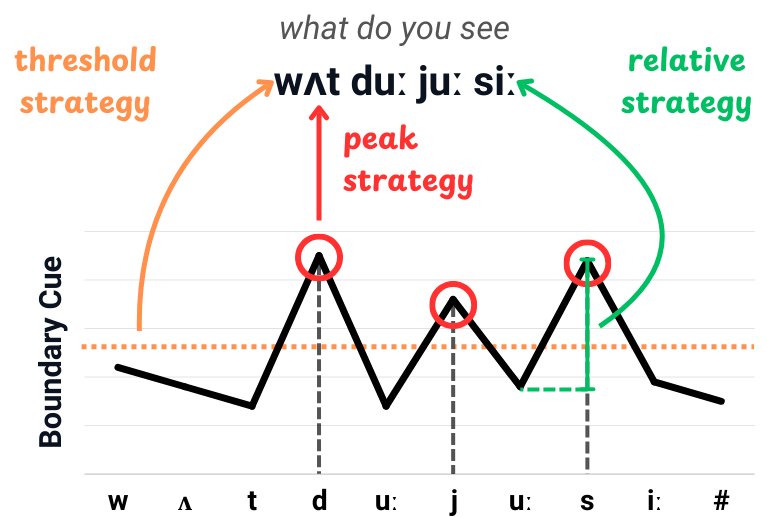
\includegraphics[width=0.95\linewidth]{Figures/15Phonology/overvieww.png}
    \caption{Three strategies for unsupervised word segmentation using cues extracted from an autoregressive language model trained to predict phonemes.}
    \label{fig:15-example}
\end{figure}

In some of the earliest sequential models, it was noted that \emph{prediction-error} (the degree to which the model struggles to predict the next token) often corresponded with word boundaries \citep{elman-1990-finding}. Using this observation,
%Noting that prediction-error in sequential models indicates word boundaries \citep{elman-1990-finding}, 
we identify four word boundary cues that can be extracted from trained models and three unsupervised strategies for placing boundaries using these cues, as illustrated in \cref{fig:15-example}. We additionally follow the supervised approach of \citet{hahn-baroni-2019-tabula}, training linear probes on final layer embeddings to determine if word boundaries are implicitly tracked in order to improve phoneme prediction.

We train phoneme-based BabyLMs on the phonemic transcriptions of child-centered speech comprising the \ipachildes dataset \citep{goriely2025}. We find that these models implicitly encode word boundaries across all 31 languages and identify two factors that may provide useful priors depending on the language: the length of words and the distribution of phonemes at the end of words. 

%but that word-final phoneme distributions and word lengths vary between languages and act as confounding factors, making it difficult to compare results across languages. 

We discuss the validity of orthographic word boundaries as gold labels and note the similarities between our results and recent work that uses byte-level prediction entropy to improve the tokenization step in large language model (LLM) pre-training \citep{pagnoni2024byte}. We conclude that this framework not only supports the study of distributional phonology and acquisition, but could also have implications for improving the efficiency and robustness of LLMs.

%Finally, we discuss the limitations of our study (\cref{app:15-limitations}) and release our code and pretrained models to facilitate future work. 

Finally, we release our code and pre-trained models to facilitate future work.

%As the training data do not contain such boundaries, this demonstrates that tracking word-like units is useful for the phoneme prediction task, suggesting that the models are learning phonological rules and providing support for statistical learning theories of acquisition. 

%We draw parallels to early neural language models, which were trained on sequences of letters or phonemes, often using developmentally plausible data in order to explore theories of word learning and phonology [citations]. For example, in the foundational work of \citet{elman-1990-finding}, a simple recurrent network (SRN) is trained to predict letters in an unsegmented sequence. Elman observes that the prediction-error increases at the onset of each new word, concluding that ``there is information in the signal that could serve as a cue to the boundaries of linguistic units which must be learned''.

%In their study, \citet{goriely2024babble} probed BabyLMs trained on the largest 11 corpora in \ipachildes for distinctive feature information. Here, we extend their work by training models on all 31 languages in the dataset and using a word segmentation task to assess their phonological capabilities.

% Through qualitative evaluation, we find that boundary placement errors are often due to the under-segmentation of common multi-word phrases and the over-segmentation of common morphemes, corroborating previous findings [citations] and contributing to discussions about how we define ``words''.

% [Little paragraph here discussing the graded notion of boundaries, and that our unsupervised method could be used to produce information-driven tokenization schemes - BLT paper? dynamic tokenization?]

% The correspondence between model prediction-error and boundaries has been observed as far back as \citet{elman-1990-finding} and could contribute to novel methods for tokenization of LLMs.

%As a zero-shot task only requires phoneme streams labeled with word boundaries (boundaries are removed in training and tested for in evaluation), which are automatically gained by grapheme-to-phoneme conversion used to generate phoneme sequences \citep{goriely2025}, this is a task that can easily be applied to any language that has these boundaries available...

%This task only requires phonemic data labeled with word boundaries and so can be easily applied to any language in \ipachildes. 

\subsection{Background}

%When trained on developmentally plausible corpora (see the BabyLM challenge, \citep{hu2024findings}), these models have demonstrated comparable performance to their graphemic counterparts \citep{bunzeck2024graphemes, goriely2024babble}.
%However, the majority of this work only considers English. Recently, \citet{goriely2025} trained phoneme LMs on child-directed speech across 11 languages, but were only able to use an English benchmark for studying how phonological and syntactic knowledge scales in phoneme LMs. 

Modern \emph{large} language models (LLMs) are still probed for grammatical information, but standard benchmarks are generally based on higher-order structures: syntax and semantics rather than morphology and phonology. 

In this work, we propose the word segmentation task as a language-independent method for probing the representations learned by phoneme LMs. Below, we summarise past approaches for investigating the phonological capabilities of language models. We then give historical background on the word segmentation task. Finally, we discuss past examples of word segmentation being used as a probing task.

Previous work has explored the representations of word boundaries in LLMs. \citet{sanabria2021difficulty} explored methods for extracting word boundaries from attention weights in an LSTM, finding that attention had limited value for segmentation. \citet{hahn-baroni-2019-tabula} trained character-level RNNs and LSTMs without word boundaries, finding that individual activations correlated with word boundaries and that a linear probe trained on all activations also identified boundaries. They claimed that removing word boundaries resulted in a `near tabula rasa' training paradigm but trained on billions of graphemic words Wikipedia, which is not developmentally plausible. Here, we use this probe on the final layer of phoneme LMs trained on developmentally plausible data, a more `tabula rasa' paradigm. 

Other studies have verified \citeauthor{elman-1990-finding}'s observations that prediction-error corresponds with word boundaries. For instance, \citet{al-rfou_character-level_2019} train a 64-layer character-level transformer and in qualitative analysis note that three measures of prediction-error sharply increase at the start of words. However, their model is trained on graphemic text from Wikipedia without removing the word boundaries and they do not explicitly use these measures to evaluate word segmentation performance. Here, we use their three measures to propose an unsupervised word segmentation algorithm using phoneme LMs trained without word boundaries.

In this study, we combine ideas from past computational models for word segmentation. Rather than explicitly calculate n-gram statistics, our cues are based on prediction-error and utterance boundary probability extracted from LLMs trained on the next-phoneme prediction task. As these cues are based on the language model's prediction of phonemes, successful segmentation indicates that implicit phonological knowledge of word-like units in these models. 

Peaks in predictability can also be observed in neural language models. In the foundational work of \citet{elman-1990-finding}, a simple recurrent network (SRN) is trained to predict letters in an unsegmented sequence (one of the first examples of autoregressive language modeling). Elman observes that the prediction-error increases at the onset of each new word, concluding that ``there is information in the signal that could serve as a cue to the boundaries of linguistic units which must be learned''.

\section{Word Segmentation Task}

% \emph{Discuss how past work has captured uncertainty in statistical models. Present the various approaches we have come up with for calculating uncertainty in LMs. Discuss the two ways that those uncertainty measures can be used to place word boundaries and the fully supervised method, using a probe or correlation calculations. Perhaps save the `increase in' measures for the appendix since they bloat the paper.}

We use the \emph{word segmentation task} as a zero-shot method for studying the phonological properties of language models trained on phoneme sequences. Given a list of utterances, each of which consists of a non-delimited phoneme sequence, the task is to produce a \emph{segmentation} of each utterance by using an unsupervised method for placing word boundaries. For instance, given the utterance ``what do you see'', represented phonemically as \ttipa{w2tdu:yu:si:}, successful segmentation would return \ttipa{w2t du: yu: si:}, as demonstrated in \cref{fig:15-example}. Note that phonemes are individual tokens (e.g. \ttipa{u:} is a single token, not two) and, crucially, word boundaries are removed during training, although utterance boundaries are present.

Our method for unsupervised word segmentation is based on the observation made by \citet{elman-1990-finding}, that cues for word boundaries can be extracted from a sequence prediction model. Given a language model that at each position $i$ provides the probability of a phoneme $x$ given a context $x_1\ldots x_{i-1}$, we extract the following four cues at each potential boundary position:

% Taking inspiration from past computational models for word segmentation, we extract three cues based on the predictability of phonemes given their context, as well as a cue based on utterance boundary prediction. Given a language model that at each position $i$ provides the probability of a phoneme $p$ given a context $p_1\ldots p_{i-1}$, our cues are as follows:

\begin{itemize}[leftmargin=*]
    \item \textbf{Entropy:} The entropy (in bits) across the probabilities for all items in the vocabulary.%\footnote{The vocabulary consists of all phonemes and a dedicated utterance boundary token.}
    \item \textbf{Loss:} The cross-entropy loss (bits) calculated as the negative log probability of the subsequent phoneme $p_i$.
    \item \textbf{Rank:} The rank of $x_i$ in the list of possible tokens at position $i$ sorted by likelihood.
    \item \textbf{Utterance Boundary Probability (UBP):} The probability assigned to the utterance boundary token.
\end{itemize}

The first three cues are put forward by \citet{al-rfou_character-level_2019}, where they are used to qualitatively examine the error rate of their character-based language model. Our use of these cues for word segmentation is novel. The fourth cue, UBP, relates to the model of \citet{christiansen1998learning}, who found that the prediction of the utterance boundary marker in a SRN increased at word boundaries. All four cues are utilized in the segmentation models of \citet{ccoltekin2014explicit, goriely2023word} but rather than being explicitly calculated using n-gram frequencies, we calculate them using the probability distribution produced by a language model.

For each of these cues, we have three methods for placing word boundaries. The first is to identify peaks in each cue: placing word boundaries whenever the cue's value is higher at position $i$ than at position $i-1$ or $i+1$ in the sequence. The second is to learn a single threshold value, placing word boundaries when the cue exceeds it. The third combines both strategies, placing word boundaries when the relative increase of the cue's value from position $i-1$ to $i$ exceeds a learned threshold. We call these the \textbf{peak}, \textbf{threshold} and \textbf{relative} strategies, respectively, as illustrated in \cref{fig:15-example}. We acknowledge that the threshold and relative strategies are not fully unsupervised, using a single learned parameter. %While threshold segmentation is not technically unsupervised, it solves an issue with peak segmentation --- the failure to place two boundaries in sequence, despite some words consisting of a single phoneme.

Finally, in order to explore whether word boundary information is present in the model's representations, we follow \citet{hahn-baroni-2019-tabula} and train a linear probe to predict word boundaries from the final layer embeddings. We implement their `balanced' probe, training on embeddings taken from an equal number of word-final and word-internal positions, and ensure that no words in the training set are contained in the test set. %Probes are trained on 1000 contextual embeddings and tested on 10,000.

% \subsection{Evaluation Metrics}\label{sec:15-evaluation}

% \emph{Briefly describe typical metrics for word segmentation and the ones we use here (likely just boundary fscore). For probe, it's either f1 or accuracy.}

\section{Experimental Setup}

We train a suite of GPT-2 models on each of the 31 languages in the \ipachildes corpus. As the size of each subset varies considerably,\footnote{The North American English section contains 10M words but Farsi only contains 40k.} for a fair comparison we must subsample our training data to the size of the smallest subset and use a very small model to prevent over-fitting. In order to explore the use of larger models and more training data, we train four suites of models, each using a different sample size and model size, setting model parameters according to the scaling experiments of \citet{goriely2025}. These suites are detailed in \cref{tab:15-suites} with parameter configurations and training parameters given in \cref{app:15-implementation_details}. The smallest model (only 2 layers) is trained on 100k tokens from all 31 languages, and the largest model (6 layers) is trained on 18M tokens of English. 

\setlength{\tabcolsep}{2pt}
\begin{table}[t]
    \centering
    \small
    \begin{tabular}{rccc}
    \toprule
        Suite Size & Model Parameters & Tokens (words) & Languages \\
       \midrule
       Tiny & 400k & 100k (\textasciitilde20k) & 31 \\
       Small & 600k & 700k (\textasciitilde180k) & 17 \\
       Medium & 5M & 1.8M (\textasciitilde500k) & 11 \\
       Large & 19M & 18M (\textasciitilde5M) & 1 \\
       \bottomrule
    \end{tabular}
    \caption{The model size in number of (non-embedding) parameters and data size used for each suite of models. Languages are subsampled according to the token count for consistency, as word length varies across languages.}
    \label{tab:15-suites}
\end{table}

For the linear probes, we follow \citet{hahn-baroni-2019-tabula} and report accuracy. They claim that chance performance is 50\% due to the balanced training data, but our results suggest otherwise. In order to evaluate our unsupervised strategies, we follow past work (see \cref{sec:15-wordseg}) compute the F1 score of boundary placement, excluding boundaries placed at the start and end of utterances (as these are `free' from the utterance boundaries).
%Past studies also report precision and recall, as well as type and token scores computed using the lexicon produced by segmentation, but it is difficult to compare scores based on the lexicon due to differences between languages.
%During training, we reserve 5000 tokens from each language to use for evaluation, kept consistent across suite sizes.
% For the linear probes, we follow \citet{hahn-baroni-2019-tabula} and report accuracy. They claim that chance performance is 50\% due to the balanced training data, but our results suggest otherwise.

\section{Experiment: Probing for phonological features}\label{sec:featureprobing}

Phoneme LMs trained on developmentally plausible corpora allow for the testing of phonological representations but recent work has only explored English models trained on 10 -- 100 million words (see \cref{sec:babylm}). Here, we establish the size requirements for models trained on data available in \ipachildes and then demonstrate how models trained on the 11 largest languages in our dataset can be used to explore emergent phonology.

We refer to the suite of models as ``cross-lingual'' as each individual model is monolingual, only trained on data from a single language. This is in contrast to ``multilingual'' models that are trained on multiple languages at once.

As the phonemic utterances in \ipachildes maintain a correspondence with \phoible, we can use the \textbf{distinctive feature} information in \phoible to probe cross-lingual phoneme LMs for phonological knowledge. 

We select the 11 largest languages in the dataset and train a GPT-2 model on each, subsampling 500 thousand words\footnote{As the number of phonemes per word varies across these languages, we actually subsample 1.8 million tokens (phonemes) for each language, which is roughly 500 thousand words.} and using the best-fitting model for this data size according to the previous experiment (the 5-million-parameter model with a dropout of 0.3). The training configuration remains the same (see \cref{sec:models}). These models allow us to compute contextual embeddings $c(x)$ for phonemes.

\begin{figure}[t]
    \centering
    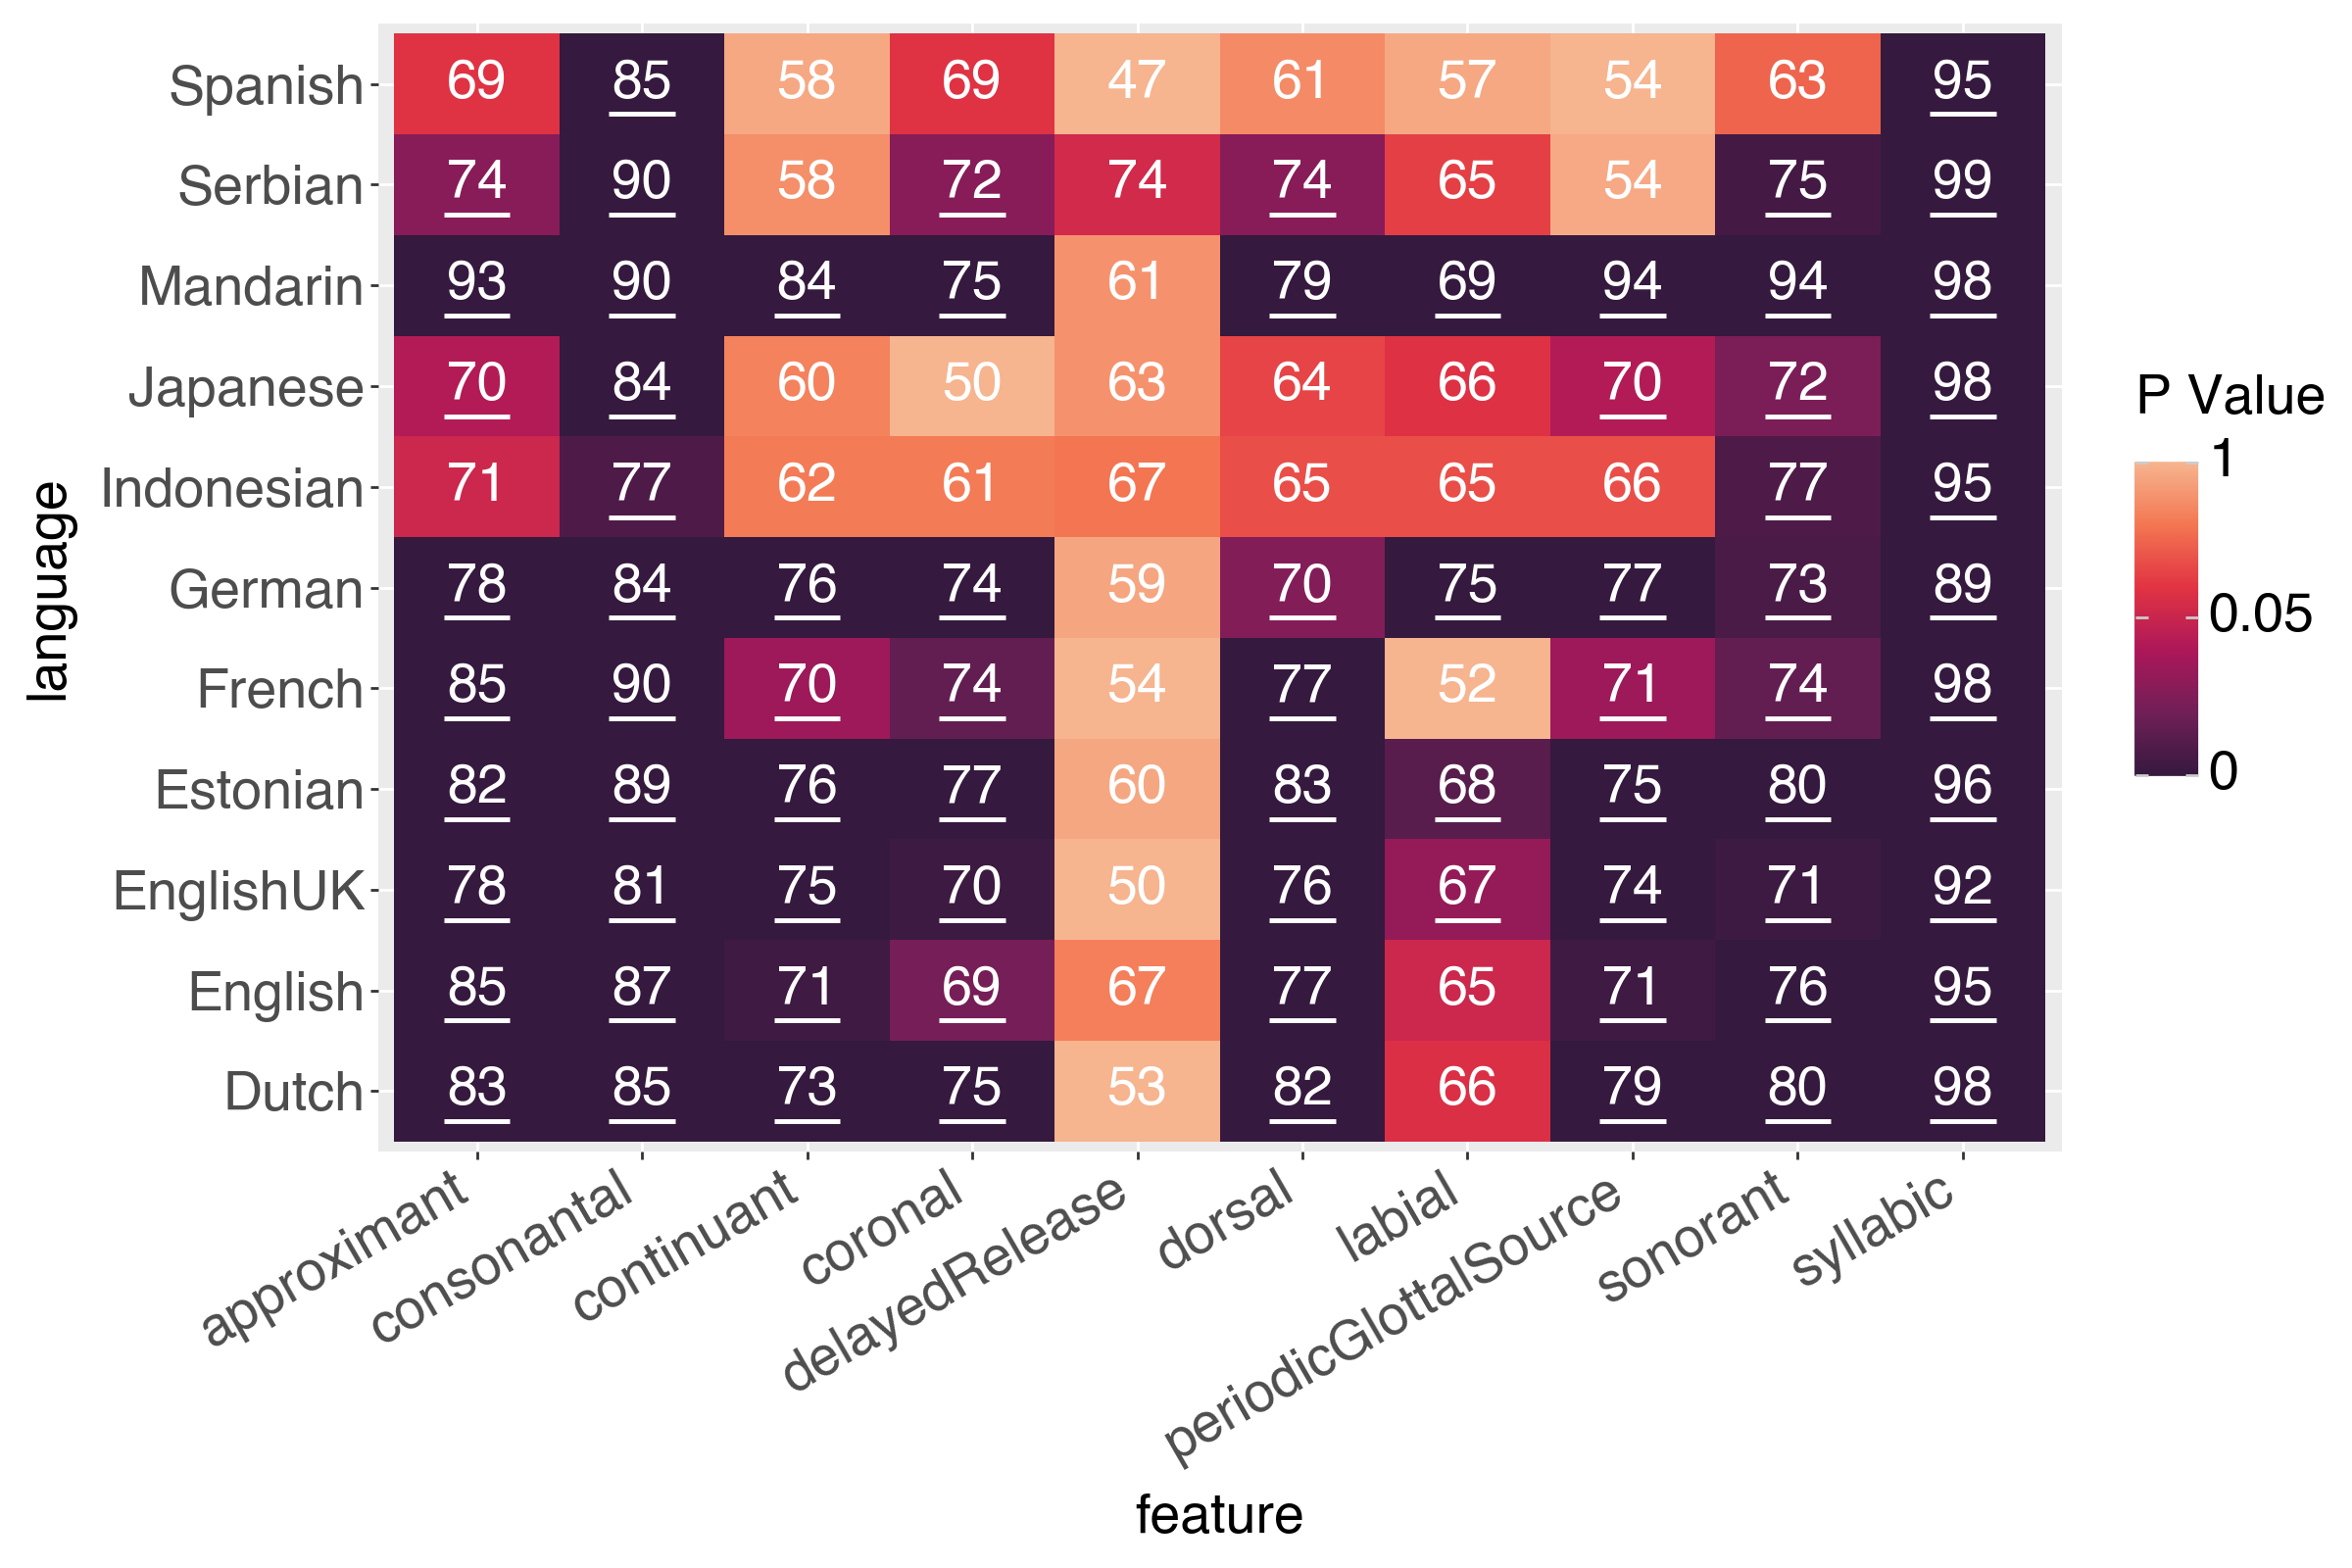
\includegraphics[width=0.99\linewidth]{15Phonology/features.png}
    \caption{Accuracy of the phonological distinctive feature probe across 11 languages in \ipachildes and 9 distinctive features from \phoible.}
    \label{fig:features}
\end{figure}

\begin{figure}[t]
    \centering
    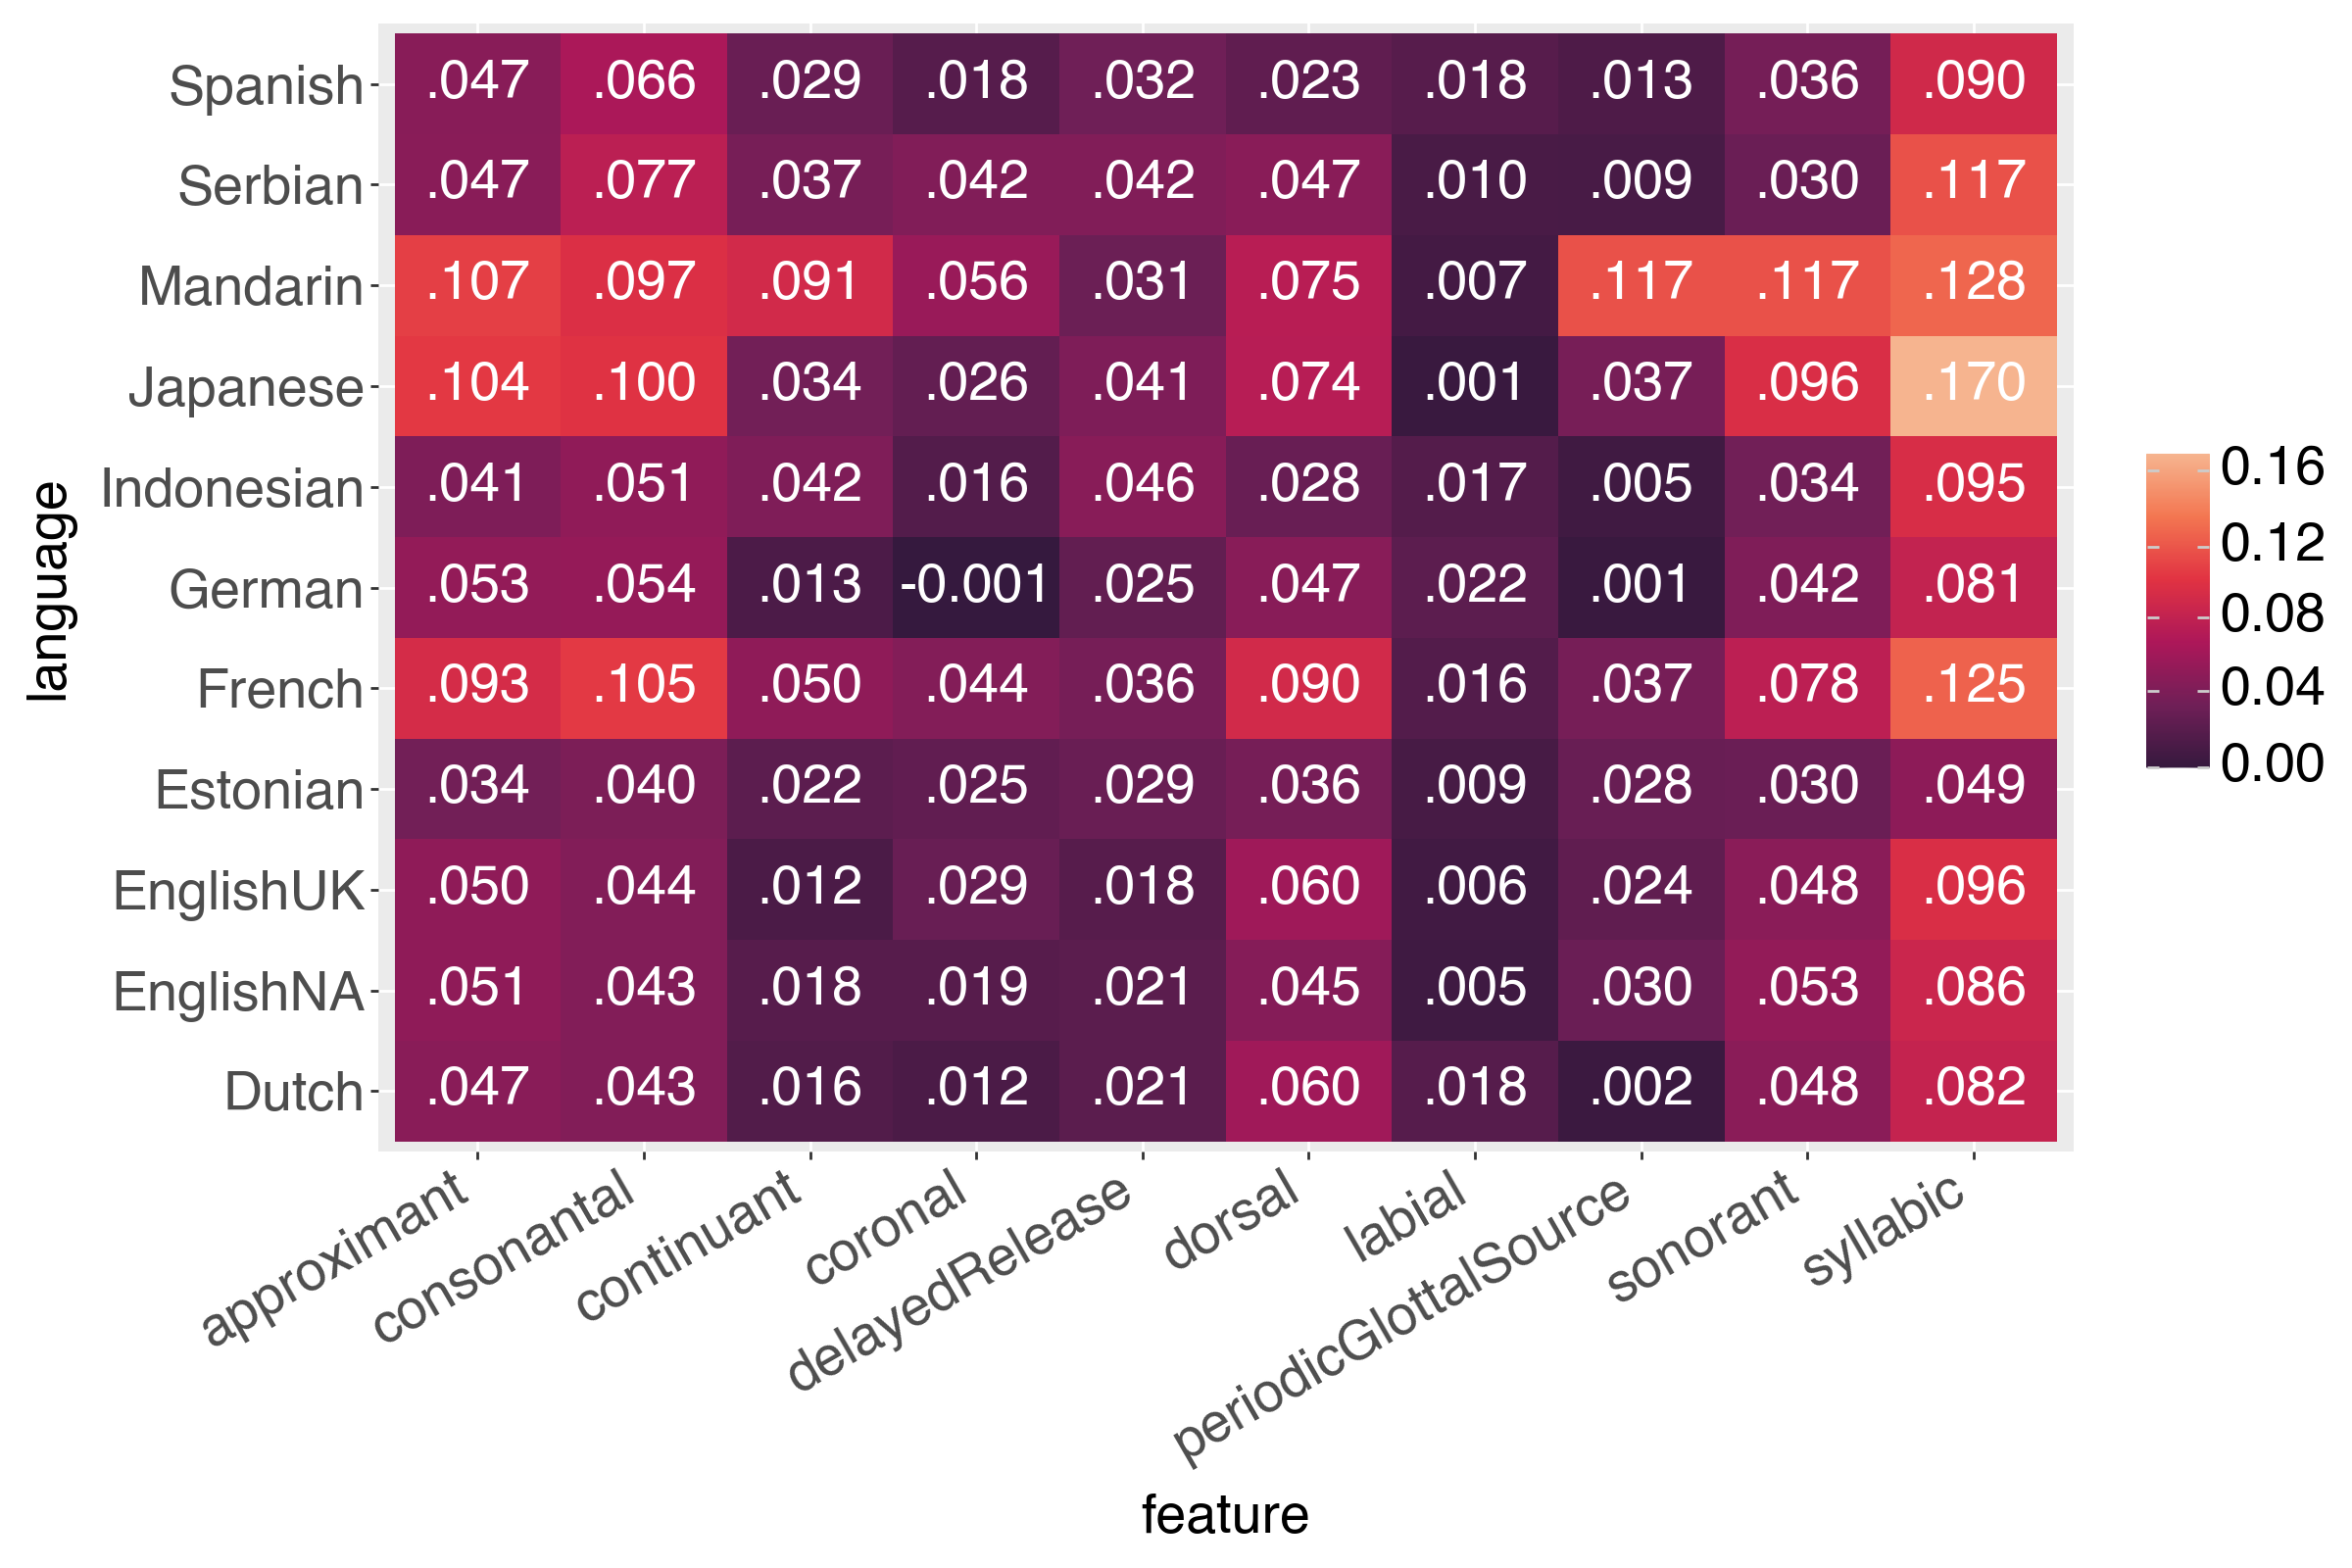
\includegraphics[width=0.99\linewidth]{15Phonology/silhouette.png}
    \caption{Average silhouette scores when using each distinctive feature to cluster contextual embeddings of the phonemes in each language.}
    \label{fig:silhouette}
\end{figure}

\begin{figure*}[t]
    \centering
    \begin{subfigure}[][][]{0.49\textwidth}
        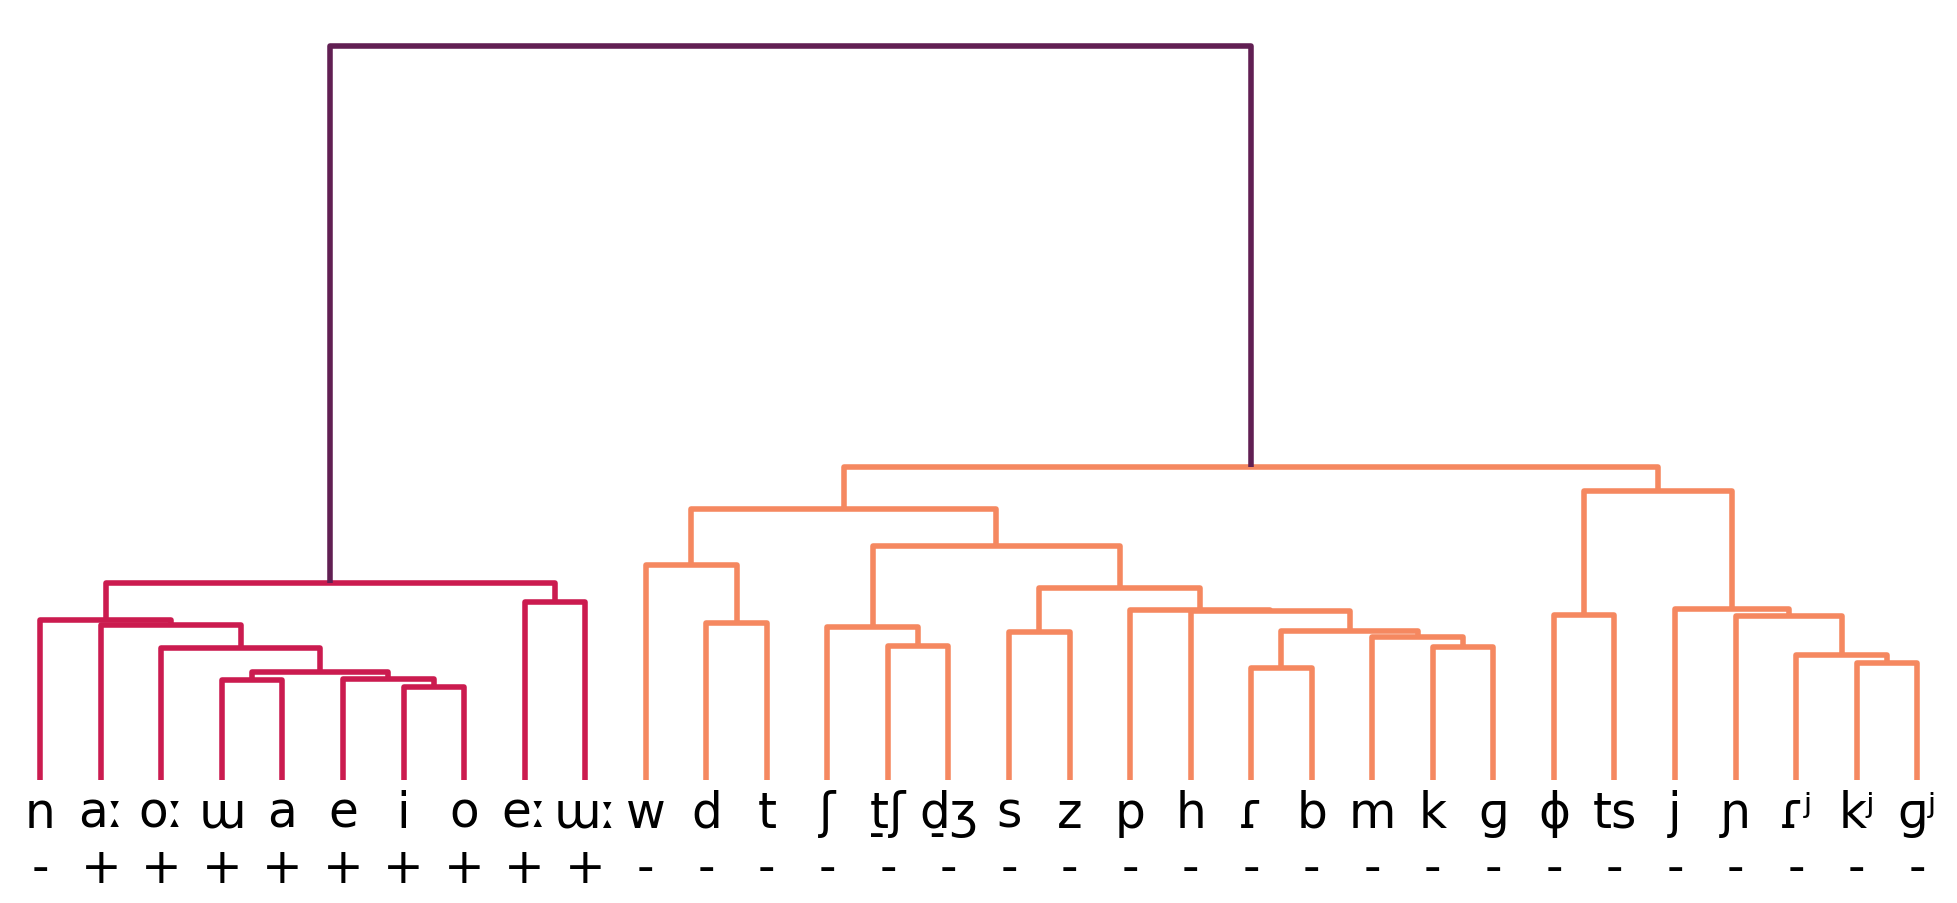
\includegraphics[width=0.99\linewidth]{15Phonology/japanesedendo.png}
        \caption{Japanese}
    \end{subfigure}
    \begin{subfigure}[][][]{0.49\textwidth}
        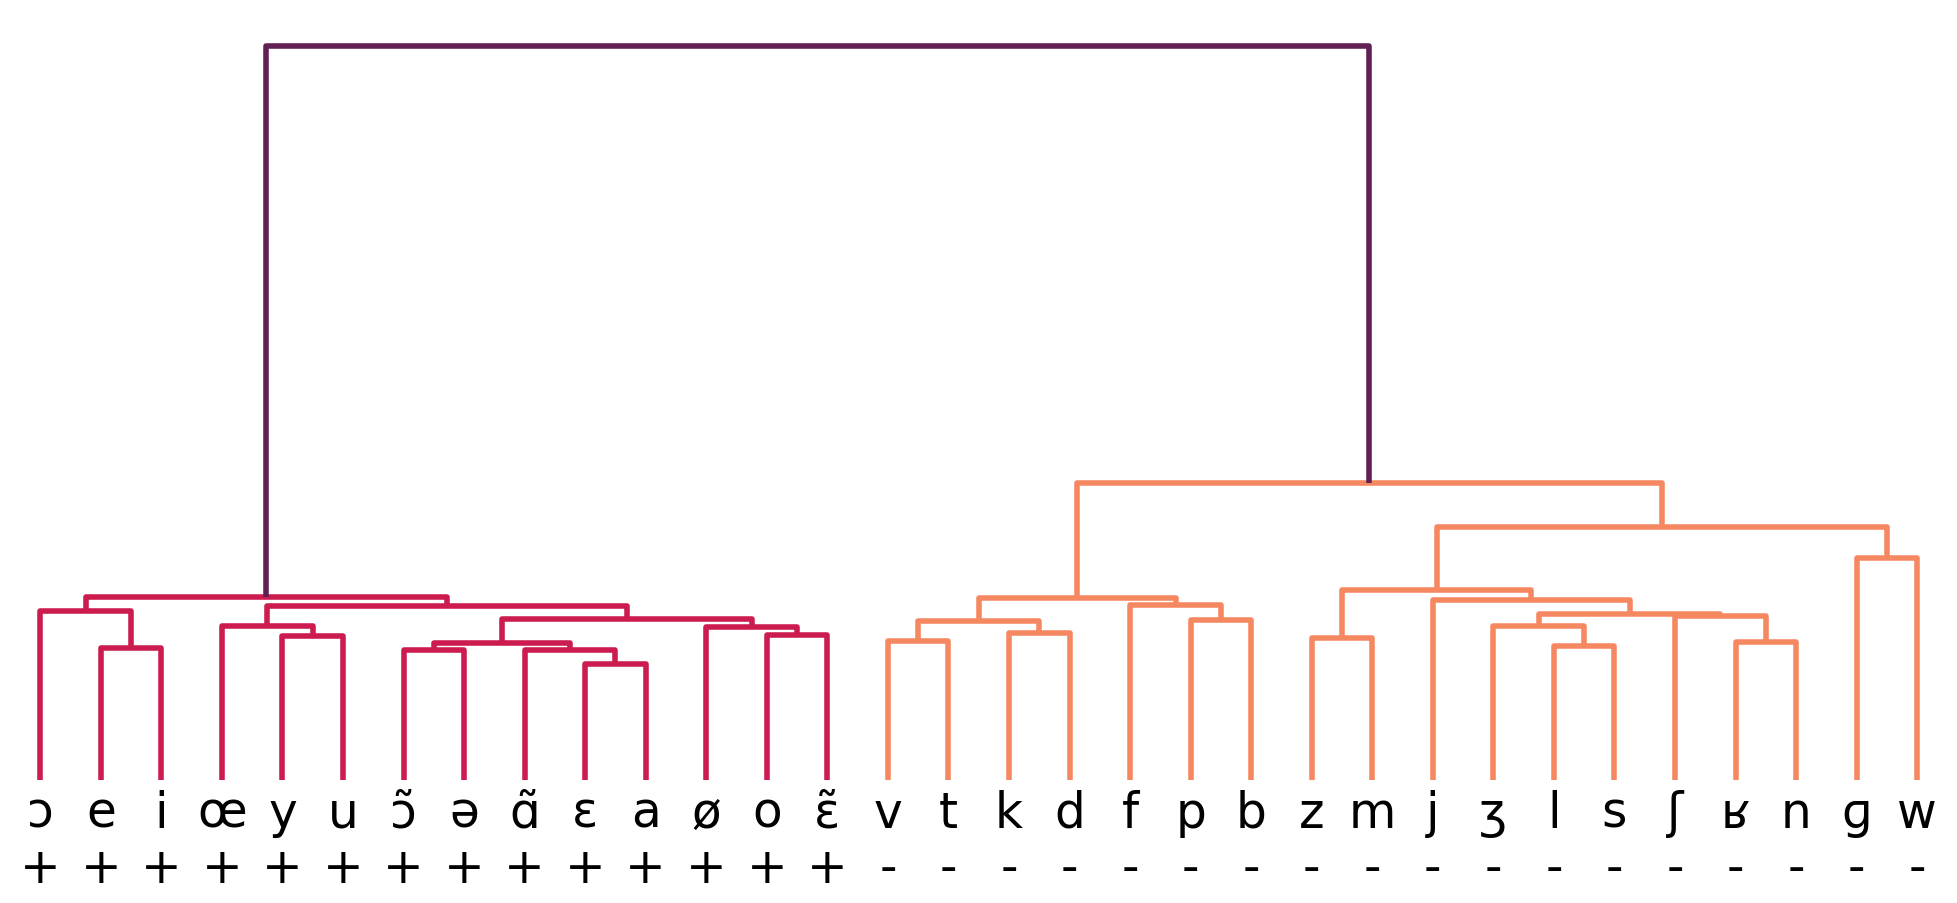
\includegraphics[width=0.99\linewidth]{15Phonology/frenchdendo.png}
        \caption{French}
    \end{subfigure}
    \caption{Similarity of the contextual embeddings for each phoneme learned by the Japanese and French phoneme LMs. Similarities are computed using Euclidean distance considering the average of 50 contextual embeddings for each phoneme and linkages are created using the incremental algorithm. The `syllabic' distinctive feature is marked below each phoneme.} 
    \label{fig:dendrogram}
\end{figure*}

We then look up the distinctive features of each phoneme in each language using the matching inventories in \phoible (see \cref{tab:13-phonemized-childes-sections}). We find the set of features for which, in all 11 languages, there are at least 4 phonemes that exhibit the feature and 4 that do not. 
For each feature $f$, we train a linear probe $p_f$ to predict that feature from the contextual embeddings $c(x)$ of phonemes. Each probe is trained with an equal number of positive and negative examples and is evaluated using leave-one-group-out cross-validation (i.e for each phoneme $x$ in the phoneme inventory $V$, the probe is trained on the contextual embeddings of all other phonemes $\{c(y) | y\in V \setminus \{x\}\}$, then evaluated by predicting the feature from contextual embeddings of the left-out phoneme $p_f(c(x))$, and the final score is a macro-average across all phonemes $x\in V$).

The results of each probe are provided in \cref{fig:features}. The majority of the probes achieve accuracies significantly\footnote{Statistical significance was assessed using a binomial test, where the null hypothesis assumes a probability of success \( p_0 = 0.5 \) and the number of trials \( n \) is equal to the number of phonemes tested by the probe. A result was considered significant if the computed \( p \)-value was less than 0.05.} higher than chance (50\%), indicating that the models learn representations that encode distinctive features. While the scores for each feature are broadly consistent across languages, some notable differences emerge. For example, nearly all feature probes achieve statistically significant results in Mandarin, whereas only two do so in Spanish. This disparity can be partly attributed to the number of unique phonemes in each language. Because we treat each combination of vowel and tone as a distinct phoneme, Mandarin has 99 phoneme types, compared to just 24 in Spanish. The smaller phoneme inventory in Spanish greatly reduces $n$ for each probe, making it more challenging to obtain statistically significant results.

In all 11 languages, the highest result is achieved by the probe for the `syllabic' feature which generally\footnote{In some languages there are also syllabic consonants, which like vowels can act as the nucleus of a syllable.} separates vowels from consonants. As these models only learn to predict phonemes and have no concept of how each phoneme is pronounced, the fact that this separation is learned clearly indicates that vowels and consonants provide a strong distributional signal across languages. The \texttt{consonantal} feature similarly separates vowels from consonants\footnote{This feature indicates an audible constriction of the vocal tract, separating obstruents, nasals, liquids, and trills from vowels, glides and laryngeal segments \citep{gussenhoven2017understanding}.} and is learned by a probe in every language. However, not every feature can be learned by these probes. For instance, the \texttt{delayedRelease} feature, which distinguishes stops from affricates, is not learned by any probe. Our models do not encode the rate of phoneme delivery, so it is unsurprising that a feature that relates to the temporal properties of phonemes is difficult to probe.

\subsubsection*{Distributional Phoneme Clusters}

To better understand why the probes capture certain phonological features, we examine whether contextual embeddings cluster according to these features. For each language, we sample 50 contextual embeddings per phoneme and label them with their associated phonological features. For each labeling, we then compute the \textbf{silhouette score} for each embedding --- a metric ranging from –1 to 1, where higher values indicate that an embedding is more similar to others in its assigned cluster than to those in neighboring clusters \citep{rousseeuw1987}. Averaging these scores across all embeddings allows us to compare how well different features cluster the phoneme representations, as shown in \cref{fig:silhouette}.

The scores are all relatively close to zero, likely due to the curse of dimensionality --- our embeddings have 256 dimensions, far exceeding the number of distinct phonemes in each language. Despite this, the results are consistent with the probe findings: the syllabic feature yields the highest clustering quality.

We further visualize this clustering using dendrograms, created by averaging the contextual embeddings for each phoneme and applying an incremental clustering algorithm. \Cref{fig:dendrogram} shows examples for Japanese and French, with the syllabic feature marked for each phoneme. In both cases, vowels are almost entirely separated from consonants, with one notable exception: \ttipa{n} in Japanese. We also observe some alignment with traditional phoneme groupings (e.g., \ttipa{b} and \ttipa{p}), though overall the dendrograms diverge from standard phonological classifications. This suggests that the distributional behavior of phonemes in context may not neatly align with their articulatory or categorical properties.

\section{Experiment: Probing for word boundaries}

% \emph{Given the range of experiments/results we'll probably want to do this section with headings corresponding to individual findings, like in the CLIMB paper. Tables might be quite big due to the number of ways to extract word boundaries. Do some language family analysis, bringing in typological features. End on an interesting experiment where maybe we use the words identified by our segmentation model to train a subword model and evaluate that on some other metric?}

\begin{figure*}[t]
    \centering
    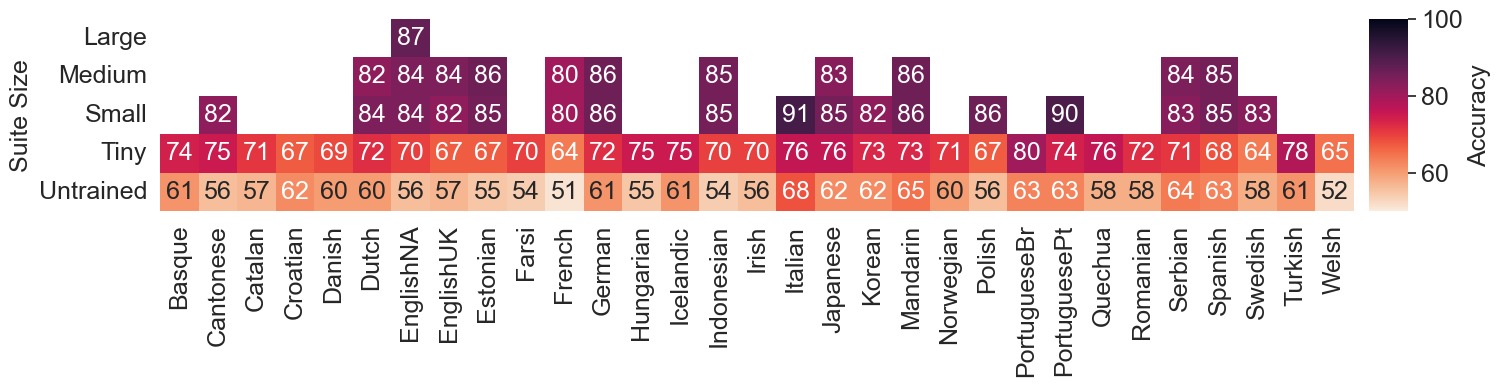
\includegraphics[width=\linewidth]{15Phonology/probe_results.png}
    \caption{Accuracy scores for the word boundary probe trained on the contextual embeddings of phonemes across models in each suite. Training and test instances are balanced and each word used for training embeddings is removed from the test set. Probe results for each untrained model in the Tiny suite are included as a baseline.}
    \label{fig:15-probes}
\end{figure*}

\begin{figure*}[t]
    \centering
    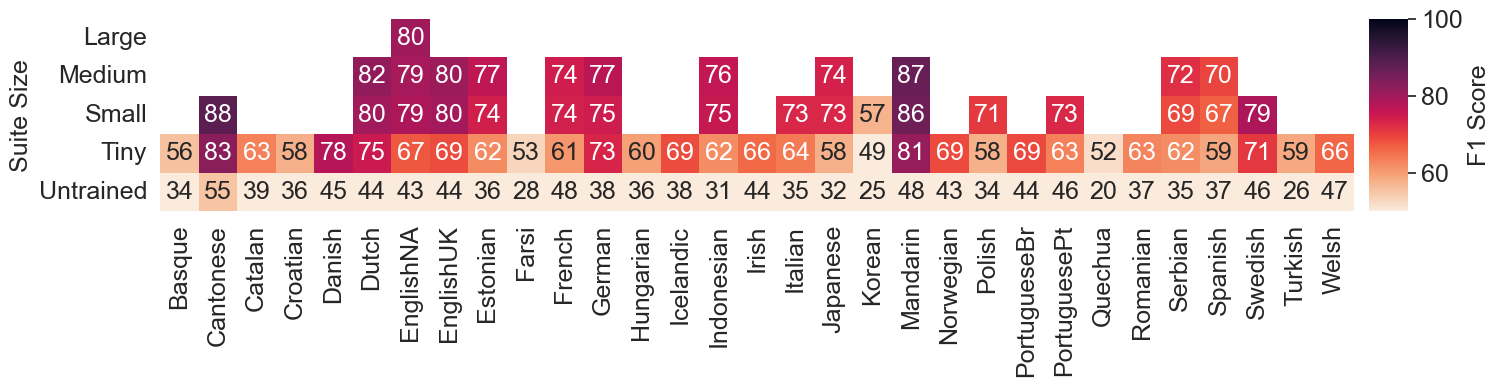
\includegraphics[width=\linewidth]{15Phonology/unsupervised.png}
    \caption{Boundary placement F1 scores achieved using the unsupervised segmentation strategies across models in each suite. For each score, we report the maximum across the 4 cues and 3 segmentation strategies. The Untrained row give the maximum scores achieved by each model in the Tiny suite before training.}
    \label{fig:15-unsupervised}
\end{figure*}

% \begin{figure*}[t]
%     \centering
%     \includegraphics[width=\linewidth]{Figures/15Phonology/small_peak.png}
%     \caption{Boundary placement F1 scores achieved by each model in the Small suite using the \textbf{peak} segmentation strategy. The ``untrained'' column give the scores achieved by each model before training, averaged across all languages.}
%     \label{fig:15-peakscores}
% \end{figure*}

We present the results of the word boundary probe in \cref{fig:15-probes} and the maximum boundary F1 scores of our unsupervised segmentation strategies in \cref{fig:15-unsupervised}. The individual scores for each combination of language, suite size, boundary cue and segmentation strategy are provided in \cref{app:15-othersegresults}. %We find that threshold correlation correlates strongly with peak segmentation (at least 0.78) and so in our analysis we focus on peak segmentation, given that it is the fully unsupervised approach and follows from past computational models. We provide full results for both strategies across suite sizes and correlation details in \cref{app:15-othersegresults}.

Overall, both the word boundary probe and the unsupervised strategies successfully identify word boundaries --- all probes achieve accuracies significantly higher than the untrained baseline, as do the unsupervised strategies (see \cref{app:15-significance} for details on significance tests). The probe accuracies show that models implicitly track word boundaries in their contextual embeddings, suggesting that they are learning phonological rules to aid in next-phoneme prediction. The unsupervised segmentation results indicate that word boundaries can be extracted through prediction across many languages, corroborating previous statistical learning results about the role of distributional cues in language acquisition.

Below, we analyse these results in more detail.

\paragraph{180k words are sufficient for learning word boundaries.}
We note that across all languages, the accuracy of the word boundary probes increases from the Tiny suite to the Small suite (where models are trained on about 180k words, as seen in \cref{tab:15-suites}), but improvements are minimal for models in the larger suites. This also occurs with the unsupervised approach, despite receiving several orders of magnitude more training data and training with many more parameters. We conclude that 180k words is sufficient for a model to learn word-like units in our framework, but other models may require more or less data. 

%We conclude that 180k words and 3 layers are sufficient for a model to learn word-like units from unsegmented transcriptions.
% MAYBE ADD SOMETHING ABOUT PAST PAPERS LOOKING AT ORDER OF ACQUISITION


%In \cref{fig:15-sizes}, we plot the F1 score achieved by the models in each suite for each language, maximizing over the score achieved by each of the four cues. For most languages, there is a larger increase from Tiny to Small than from Small to Medium, but there are some exceptions. For instance, the largest performance increase for the German models occurs between the Small and Medium sizes. Meanwhile, the probe achieves the same accuracy of 86 for both. This indicates a discrepancy between the extent to which word boundaries can be extracted from contextual representations compared to being extracted from probability distributions produced by the model, which may become more stable with larger model sizes and training data availability.

% \begin{figure}[t]
%     \centering
%     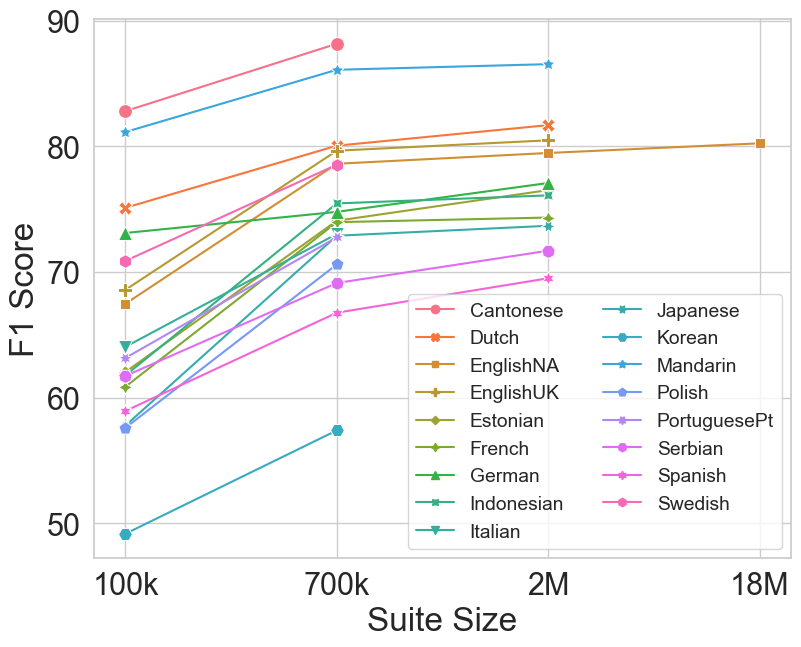
\includegraphics[width=\linewidth]{Figures/15Phonology/sizes.png}
%     \caption{Maximum boundary placement F1 scores achieved by each model across suite sizes. Only languages that appear in at least two suites are included.}
%     \label{fig:15-sizes}
% \end{figure}

% \begin{figure}[t]
%     \centering
%     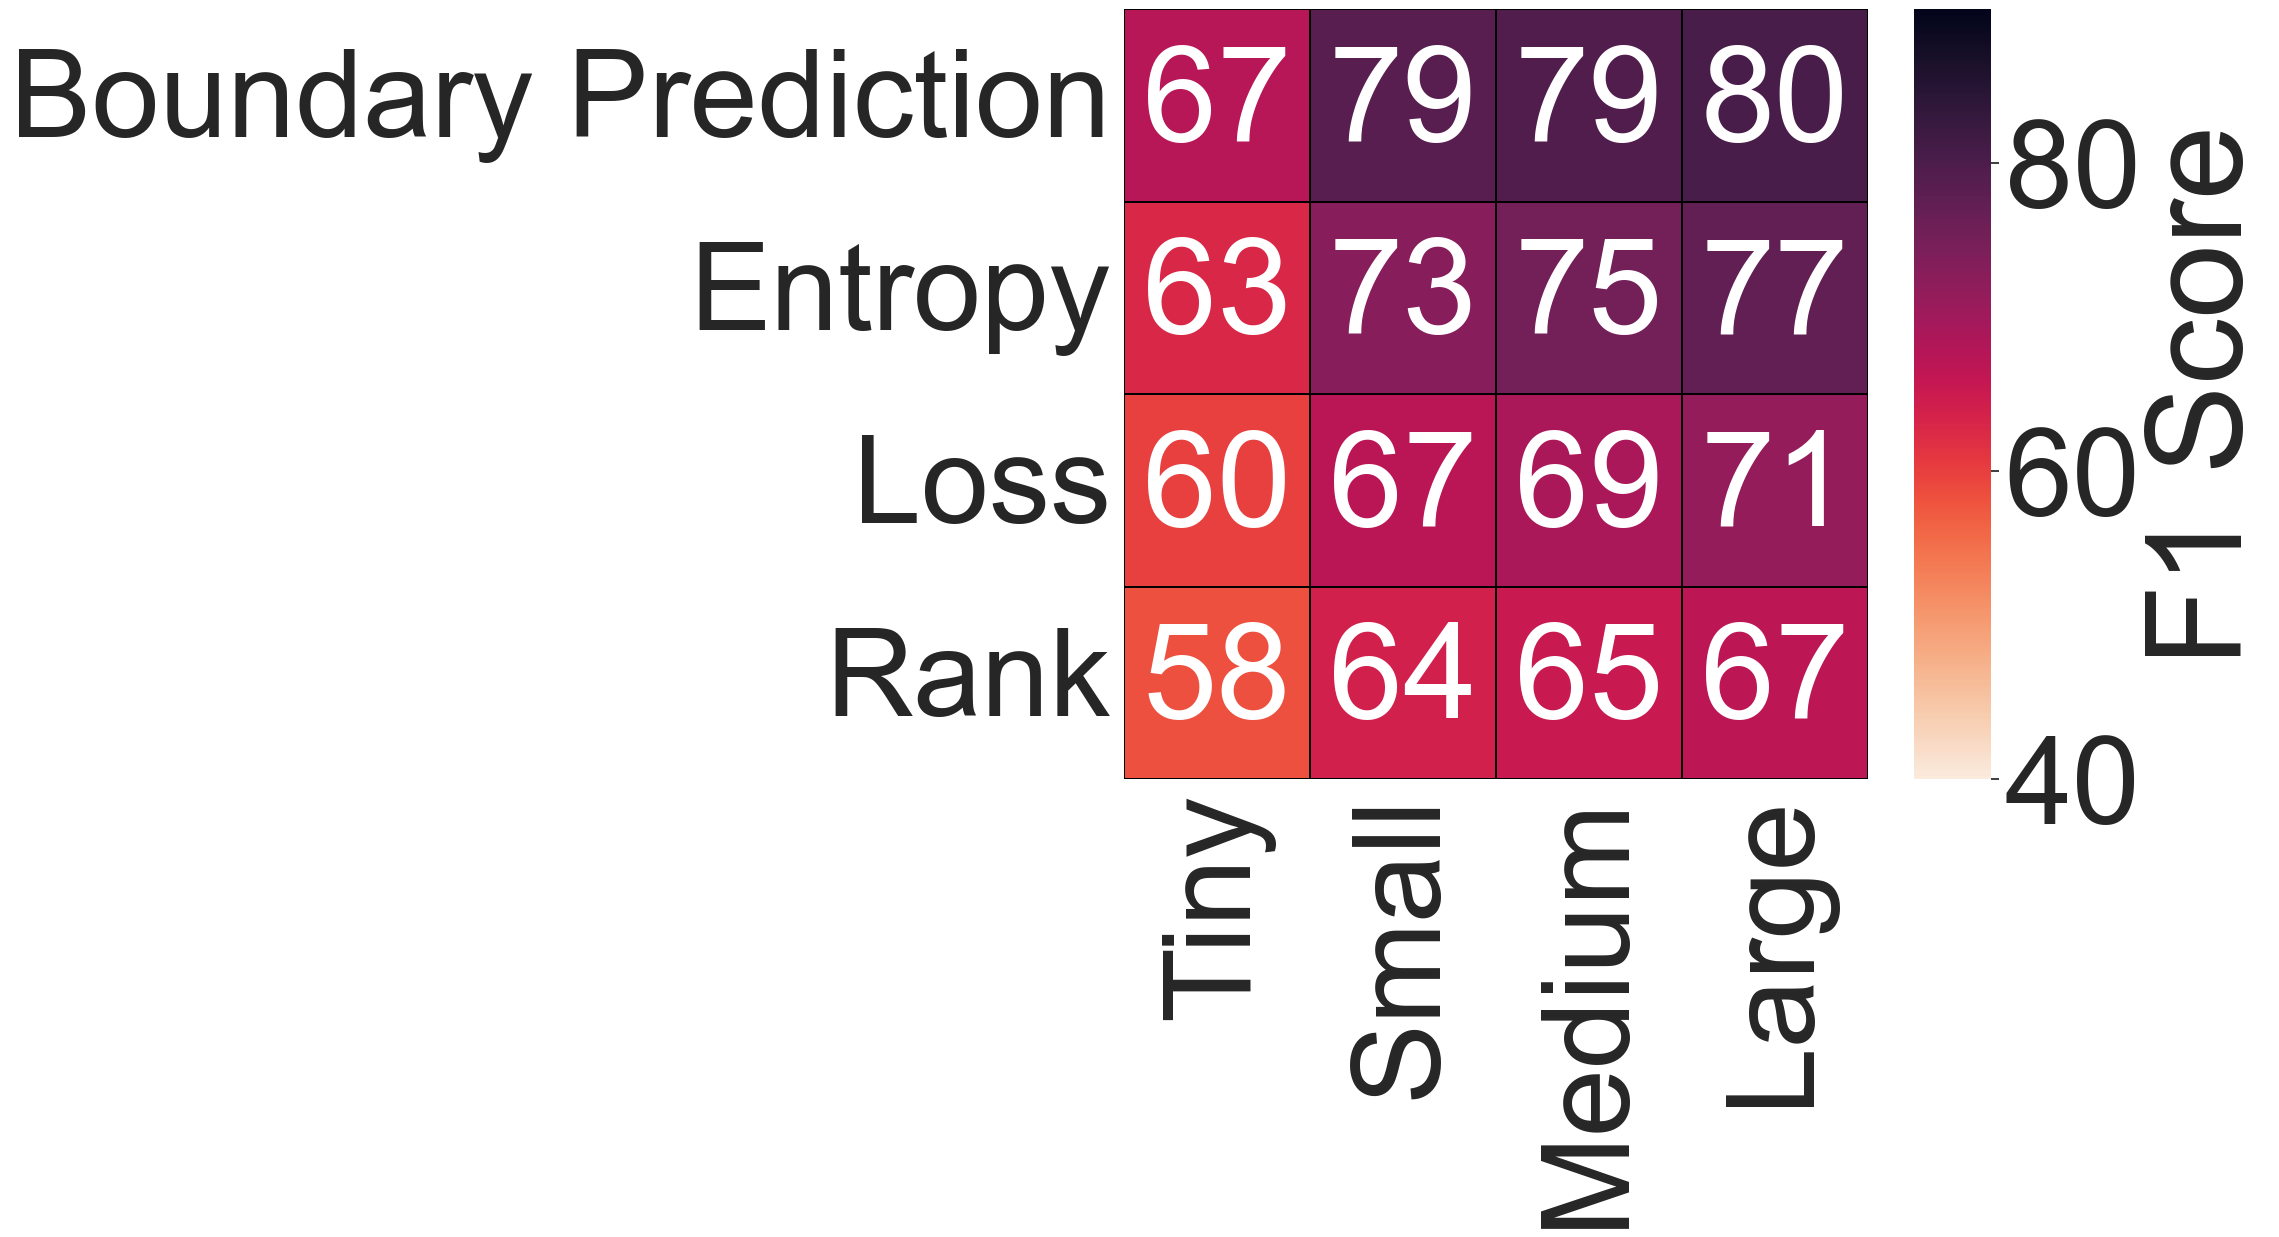
\includegraphics[width=\linewidth]{Figures/15Phonology/english_growth.png}
%     \caption{Boundary placement F1 scores achieved for the English model using the \textbf{peak} segmentation strategy across suite sizes.}
%     \label{fig:15-englishgrowth}
% \end{figure}

\paragraph{Utterance boundaries are better predictors of word boundaries than prediction-error.}
\Cref{fig:15-unsupervised} provides the maximum boundary F1 score achieved for each model in each suite across the four boundary cues and three segmentation strategies, for a total of 12 combinations. In \cref{tab:15-bestcues} we summarize the cue and strategy combinations that achieved these scores. The UBP cue is the most effective in each suite, out-performing the three cues based on prediction-error, and the relative strategy out-performs the other two strategies. For reference, we give the best combinations for each language in \cref{app:15-othersegresults}. Generally, the best cue stays consistent across suites for a particular language (e.g. Entropy is the best cue for Italian), but this is not always the case, and the best strategy also varies. %[More analysis here]

\begin{table}[]
    \centering
    \small
    \begin{tabular}{lcccc}
    \toprule
    Cue \& Strategy & Tiny & Small & Medium & Large \\
    \midrule
    UBP (threshold) & 3 & 2 & 1 & - \\
    UBP (relative) & 3 & 6 & 4 & - \\
    UBP (peak) & 11 & 4 & 3 & 1 \\
    Entropy (threshold) & 1 & - & 1 & - \\
    Entropy (relative) & - & 4 & 2 & - \\
    Entropy (peak) & - & 1 & - & - \\
    %Loss (threshold) & - & - & - & - \\
    Loss (relative) & 9 & - & - & - \\
    %Loss (peak) & - & - & - & - \\
    %Rank (threshold) & - & - & - & - \\
    Rank (relative) & 3 & - & - & - \\
    Rank (peak) & 1 & - & - & - \\
    \bottomrule
    \end{tabular}
\caption{Counts of the word boundary cues and segmentation strategies that achieved the highest F1 scores in each suite.}
\label{tab:15-bestcues}
\end{table}

%We compare four cues for our unsupervised word segmentation strategy, one based on utterance boundary probability and three based on prediction-error. Examining the Small suite peak segmentation results in \cref{fig:15-peakscores}, we find that the Boundary Prediction cue achieves the highest F1 score for 13 of the 17 languages. Of the three prediction-error cues, Entropy scores higher than Loss or Rank for 15 of the 17 languages.

\paragraph{The peak segmentation strategy fails to capture subsequent boundaries.}
We compare the four segmentation cues using the peak strategy segment utterances from the EnglishNA section of \ipachildes in \cref{fig:15-qualitative}. We identify two failure modes for this strategy. The first is that since two peaks cannot directly follow one another, subsequent boundaries cannot both be successfully placed. In this example, the \ttipa{h} in ``help'' is incorrectly placed by all four cues. A second failure case is that the relative size of peaks is not considered; three cues incorrectly place a boundary within the word ``fingers'' due to a very small peak at \ttipa{\textschwa}. The threshold and relative segmentation strategies address both of these issues but for English the peak strategy is still best overall.

% SEE \cref{app:15-qualitative})

\begin{figure*}
    \centering
    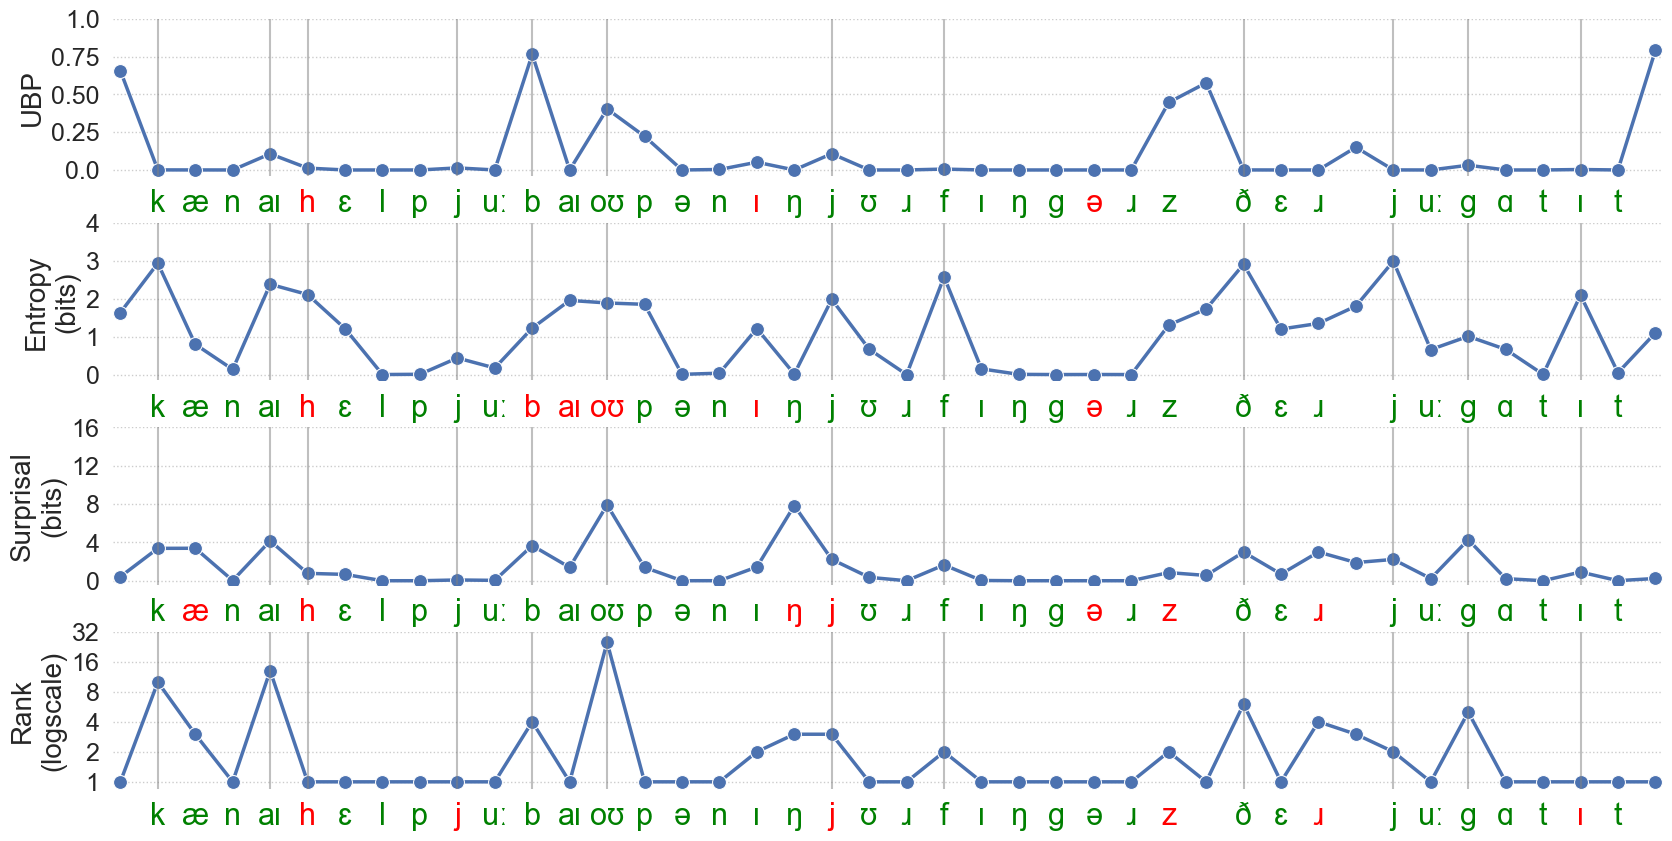
\includegraphics[width=\linewidth]{Figures/15Phonology/qualitative.png}
    \caption{Per-phoneme boundary probability, entropy, loss and rank assigned by the Medium English model for the sequence of utterances ``can I help you by opening your fingers'', ``there'', ``you got it''. Spaces indicate utterance boundaries, vertical lines indicate gold word boundaries and phonemes are marked as green if they are correctly identified as word boundaries using the \textbf{peak} strategy or if they follow an utterance boundary (red otherwise).}
    \label{fig:15-qualitative}
\end{figure*}

% \emph{Qualitative evaluation of the English model is given in \cref{fig:15-qualitative}. First, we note one of the failure cases for the peak segmentation strategy. Since by definition one peak can't follow another, the \ttipa{h} in ``help'' cannot be correctly identified as a word boundary for any measure after preceding \ttipa{aI} is correctly identified.}

% \emph{Considering the relatively longer words ``opening'' and ``fingers'', we see that when segmenting with the Boundary Probability or Entropy cue, the `incorrect' bondaries split the words into possible morphoneme, ``open''+``ing'' and ``fing'' + ``ers''. This last segmentation is barely visible on the plot and this segmentation probably should not happen given that `e` appears 99.9\% of the time after `fing` in the training dataset, but since the strategy only captures relative certainty, we incorrectly place a word boundary. }

\begin{figure}[t]
\centering
\begin{subfigure}{0.95\linewidth}
    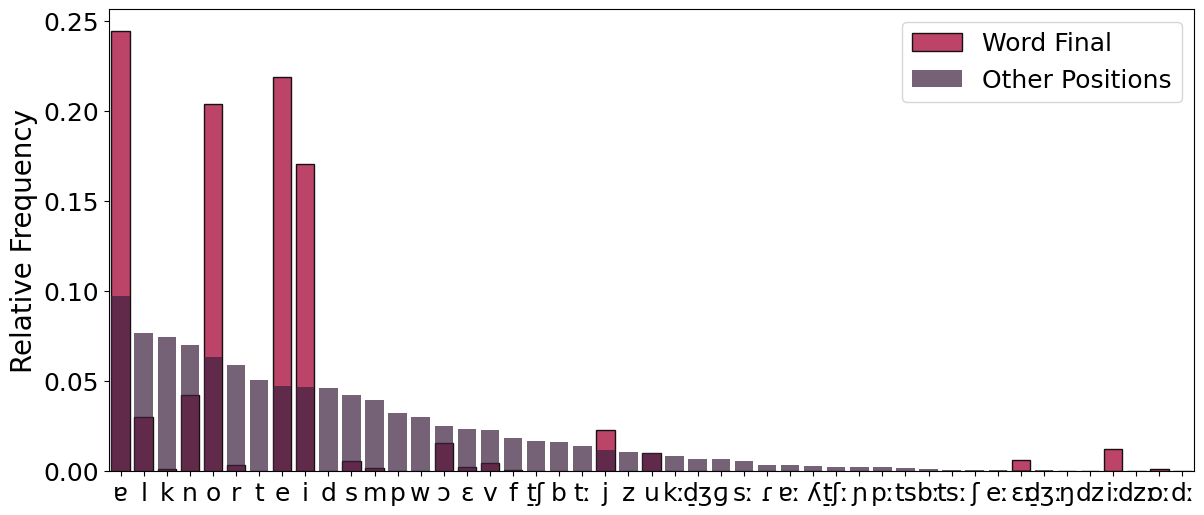
\includegraphics[width=\linewidth]{Figures/15Phonology/italian.png}
\end{subfigure}
\hfill
\begin{subfigure}{0.95\linewidth}
    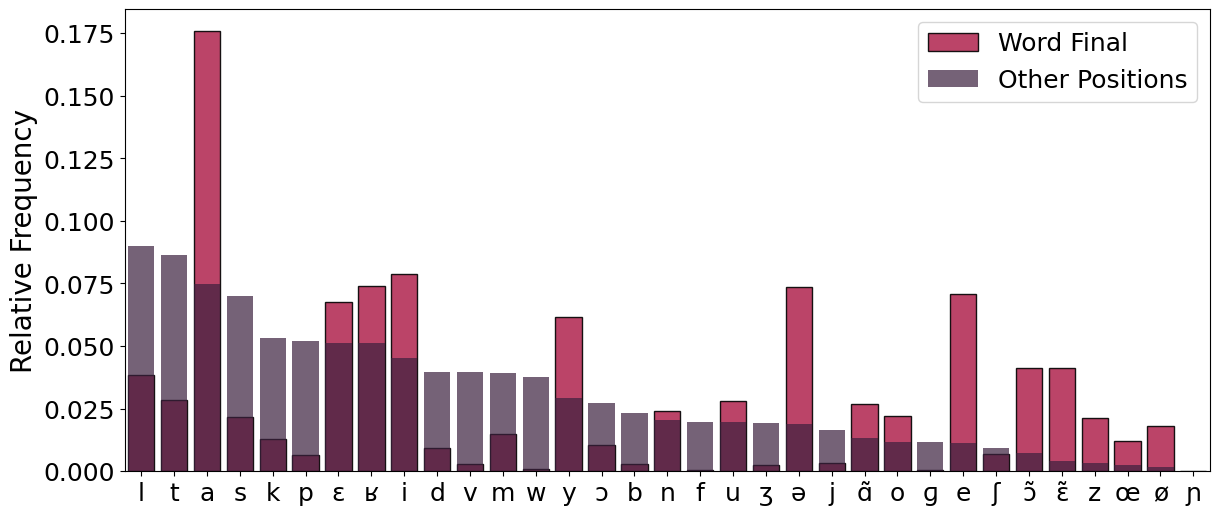
\includegraphics[width=\linewidth]{Figures/15Phonology/french.png}
\end{subfigure}
\hfill
\caption{Relative frequencies of phonemes appearing in word-final positions and all other positions for Italian (top) and French (bottom).}
\label{fig:15-frequencies}
\end{figure}

%the same number of word-final embeddings, labeled as boundary positions, as the number of non-word-final embeddings
%they must identify word-final contextual embeddings, with all other positions labeled as non-boundary
%where the the number of word-final embeddings used to train the probe is equal to the number non-word-final embeddings

\paragraph{Italian has a strong prior for learning word boundaries.}
\citet{hahn-baroni-2019-tabula} claim that since the probes are trained on balanced examples,
chance accuracy should be 50\%. However, we find that the probes trained on completely untrained models (see \cref{fig:15-probes}) achieve accuracies ranging from 51\% for French up to 68\% for Italian. This is because the balancing procedure does not account for the fact that phonemes have different probability distributions depending on their position within words. For example, in \cref{fig:15-frequencies} we find that at the end of Italian words, a small number of phonemes have particularly high frequencies (the vowels \ttipa{\textturna, o, e} and \ttipa{i} end 84\% of words) whereas the distribution of French word-final phonemes is not as skewed. This skewed distribution provides a useful prior for the Italian probe, which can achieve high accuracies by relying on these phoneme frequencies (the only signal available when using embeddings from an unsupervised model). To measure the relative benefit of each prior, we can compute the \textbf{normalised entropy} of the word-final phoneme distributions in each language, 

$$H_\mathrm{norm}=\frac{H(P)}{H_\mathrm{max}} = \frac{\sum_{i=1}^np_i\log_ip_i}{log_2(n)},$$ 
which ranges from 0 (deterministic distribution) to 1 (uniform distribution). We find that not only do Italian and French have the lowest and highest normalised entropies with 0.51 and 0.84, respectively, but in general, this normalised entropy has a high negative correlation with probe accuracy for the untrained models (Pearson $\rho = -0.69$). This correlation is still present for the Tiny suite (Pearson $\rho = -0.52$) but is not significant for the Small and Medium suites, indicating that although the word-final phoneme distribution prior is useful, the embeddings do still encode information about word boundaries that the probes can detect.

%This finding indicates that the word segmentation task may be inherently easier for some languages than others when relying solely on distributional information.  he Italian probe does perform the best in each suite, however still significantly improves over its baseline, indicating that the model is still learning to track boundaries. 

%We can measure how skewed the word-final distributions are by computing the entropy of the word-final phoneme distributions and normalizing it (dividing by $log(n)$ where $n$ is the number of phonemes for that language). This gives a score between 0 and 1 for each language where 0 indicates a deterministic distribution and 1 indicates a uniform distribution. We find that not only do Italian and French have the lowest and highest relative entropies with 0.51 and 0.84, respectively, but in general, this relative entropy has a high negative correlation with probe accuracy for the untrained models (spearman -0.70). This correlation drops to -0.48, -0.47 and -0.09 for the Tiny, Small and Medium suite results, the last two of which are not significant, presumably because as the models grow they learn more sophisticated distributional patterns that the probe can use to its advantage.
%suggesting that once the models reach a certain size they are learning distributional patterns more sophisticated than simple phoneme frequency. 


\paragraph{Word length is a confounding factor for unsupervised segmentation.}
Just as with the probes, using our unsupervised methods on untrained models can reveal confounding factors, as shown in \cref{fig:15-unsupervised}. The F1 scores for the untrained models range from 20 for Quechua up to 55 for Cantonese. For 25 of the 31 languages, this score comes from the UBP cue with the relative strategy; since the probability of an utterance boundary from an untrained model will randomly vary over the phoneme sequence, boundary placement using the relative strategy essentially places boundaries randomly, which can still yield relatively high F1 scores if words are short. This seems to be the case here; Quechua has the highest average word length in \ipachildes and Cantonese has the lowest, with 6.2 and 2.4 phonemes per word, respectively. Generally, we find that word length has a high negative correlation with the F1 scores with Pearson $\rho = -0.94, -0.71, -0.79, -0.42$ for the Untrained, Tiny, Small and Medium suites, respectively (although the final correlation is not significant). 

This confounding factor means that we cannot easily compare word segmentation scores between languages, only scores for each language across suite sizes. Compared to the untrained models, the unsupervised word segmentation strategy still achieves significantly higher F1 scores for every language, demonstrating that distributional information is a useful cue for bootstrapping a lexicon. 

% \emph{Past computational models of word segmentation have mostly focused on English. In their multilingual study, \citet{goriely2023word} found that English achieved one of the highest boundary F1 scores. Here, English does perform relatively well for unsupervised segmentation but not necessarily for the probe, where for the Tiny suite English is on the lower end. On the other hand, unsupervised segmentation with the Korean model...}

\section{Discussion}

In this work, we train BabyLMs on phonemic transcriptions of 31 languages in \ipachildes and explore the word segmentation task as a method for probing these models for phonological knowledge. Our results indicate that prediction-error and utterance boundary probability can be used as cues for unsupervised word segmentation. Our study is the first to use prediction-error extracted from LLMs for unsupervised word segmentation, extending previous work that explicitly calculated these cues using n-gram models \citep{ccoltekin2014explicit, Coltekin2017, goriely2023word}. We also update previous neural models of word recognition \citep{elman-1990-finding, christiansen1998learning} by using modern architectures and evaluating cross-lingually. We now turn to the broader implications of our findings.

\paragraph{Statistical learning.} Viewing our models as statistical learners, we find that no single cue or strategy consistently yields the best segmentation performance across different model sizes and languages. This is perhaps unsurprising, as many of the cues are highly interrelated (for example, entropy and surprisal often correlate) and all segmentation strategies are grounded in the same underlying principle: identifying boundaries at points of high prediction uncertainty. It is this general principle, rather than any specific cue or strategy, that proves sufficient for segmenting utterances into word-like units. Nevertheless, most cues and strategies perform reasonably well on their own. Previous segmentation models have explored combining multiple distributional cues through unsupervised majority voting \citep{Coltekin2017, goriely2023word}, an approach that could be fruitfully applied to the cues investigated here in future work.

\paragraph{Cross-lingual comparison.} Comparing models across languages is a challenge. Our study is the first cross-lingual study using the word segmentation task to compare 31 languages, but we identify two confounding factors that inhibit cross-lingual comparison. Firstly, we find that the distribution of phonemes in word-final slots provides a prior not previously accounted for in studies that probed contextual embeddings for word boundary information. Secondly, we find that word length provides a prior for the unsupervised strategies, since randomly placing boundaries yields a higher F1 score when words are shorter, which has not previously been accounted for in cross-lingual word segmentation studies. Nevertheless, both the probes and the unsupervised strategies achieve significant scores for all 31 languages, indicating the importance of the distributional cue for learning to segment speech in any language. These findings also highlight the importance of accounting for frequency information as a prior when training probes or comparing models trained on different datasets.

\paragraph{Simulating acquisition.} Our results focus on the performance of our models at the end of training, whereas past work has compared the learning dynamics of phoneme-based models to developmental patterns observed in human acquisition \citep{kirov-2018-recurrent}. Although our findings indicate the utility of the distributional cue for identifying word-like units, we do not claim that our models simulate language acquisition. In particular, given recent advances in models that operate directly on raw audio, the use of phoneme-level representations may be insufficient for capturing the full complexity of language learning, as discussed in \cref{app:limitations}.

Rather, we use this framework to investigate the distributional patterns of phonemes across languages and whether language models trained to predict upcoming phonemes implicitly track meaningful sub-sequences that align with words. While many computational models of word segmentation treat segmentation as a necessary precursor for language understanding, this assumption has been questioned. For example, \citet{Baayen02012016} show that a tri-phone model, operating on unsegmented utterances can make predictions consistent with infants' sensitivity to linguistic structure. Likewise, recent phoneme-level language models perform well on both linguistic benchmarks and downstream tasks without explicit segmentation \citep{goriely2024babble} --- although our results suggest that some degree of implicit segmentation may be occurring to enhance these models' predictive performance. 

\paragraph{Word boundaries as gold labels.} Throughout this work, we have used word boundaries from orthographic text as the gold labels for evaluation, but these boundaries may not correspond with lexical units in speech. In early stages of acquisition, children may treat both predictable multi-word phrases as single lexical units \citep{macwhinney1978} and unsupervised word segmentation strategies may be segmenting morphemes, rather than words \citep{fleck2008lexicalized}. From an information-theoretic angle, word boundaries may only exist to optimize the trade-off between syntax and morphology across languages \citep{koplenig2017statistical, mosteiro2025word} and in general, what exactly defines a `word' is still up for debate \citep{dixon2002word, haspelmath2023defining}. 

\paragraph{Unsupervised segmentation for tokenization.} Instead of evaluating against word boundaries, we can treat our cues as \emph{graded} measures of co-occurrence statistics, as noted by \citet{elman-1990-finding}. This idea can be leveraged to improve the tokenization step in modern LLM pre-training. Instead of forming subwords by merging frequently occurring byte pairs, token sequences that are highly predictable can be combined. \citet{pagnoni2024byte} apply this concept to a ``token-free'' model, where bytes are joined into `patches' according to the entropy of the probability distribution for each byte (probabilities are computed using a byte-level LLM). They use two constraints for merging bytes which exactly correspond to our threshold and relative segmentation strategies, but only use entropy as a cue. In our experiments, entropy was less effective than utterance boundary probability (UBP) for unsupervised word segmentation and in an initial investigation (see \cref{app:tokenizers}) we found that creating a subword tokenizer using both cues improves the linguistic abilities of models trained on phonemes compared to regular BPE and that the UBP cue is more effective than entropy. This creates a parallel between word segmentation research and practical applications for tokenization in NLP and we encourage further work in this area.



%which we found to be inferior to utterance boundary prediction and model loss for unsupervised word segmentation. In an initial investigation (see \cref{app:15-tokenizers}), we found that tokenizers based on these cues improve the linguistic abilities of models trained on phonemes over regular BPE, creating a link between word segmentation research and tokenization in NLP. We encourage future work to further explore the use of these cues to improve tokenization.

%larger-scale information-driven tokenization schemes. 

% \subsection{Comparison to past models of Word Segmentation}

% Past computational models of word segmentation typically evaluate their approaches on the BR corpus, which consists of just under 10,000 utterances originally collected by \citet{bernstein1987phonology}, stored in the EnglishNA portion of CHILDES and transcribed phonemically by \citet{Brent1999}. It consists of 96k phonemes, similar in size to our Tiny suite. Many models are evaluated `online', segmenting each utterance as its contents are also used to update the segmentation model, rather than learning statistics first, then evaluating. Boundary placement F1 scores for state-of-the-art models of word segmentation vary from 82 to 90 on this corpus (see \citet{goriely2023word} for a detailed comparison of past models). Clear that using transformer models and extracting uncertainty from predictions requires more data, but 200k still very reasonable compared to the scales that LMs are typically trained on.


% \subsection{Word Boundaries}

% \emph{Discuss the notion of a `word' across languages in relation to what we've found here.}
% \emph{Brief discussion about whether using orthographic word boundaries as the gold is valid, mention previous discussions about words and cite Elman again. Also mention that here we use utterance boundary prediction as a cue for word boundaries, following early work etc.}

% IMPORTANT: Possibly note Elman's reluctance to call this a model of word learning due to other cues... Also Elman neatly discusses that boundaries are graded.

% \subsection{Multilingual Language Modeling}

% \emph{Past word segmentation models primarily focus on English and perhaps one or two other languages. Here we train on 31 from CHILDES. \citet{caines2019cross} and \citet{goriely2023word} are similar studies, doing 28 languages, but not using LLMs. Our models could also help with low resource language modeling research etc.}

% \subsection{Model Uncertainty}

% \emph{Potentially discuss work to do with extracting `uncertainty' aka confidence from language models. Not as directly relevant as the other work but is more mainstream in current NLP terms.} 

\section{Conclusion}

Phoneme-level language models trained on developmentally plausible corpora are a valuable tool for studying cross-lingual phonology and theories of acquisition. In this study, we demonstrate how the \textbf{word segmentation task} can be used to probe these models for phonological knowledge and introduce novel unsupervised methods leveraging prediction-error and utterance boundary probability to identify words. Our findings show that models trained on 31 languages can all detect word boundaries; however, cross-linguistic comparisons are influenced by confounding factors such as word length and word-final phoneme distribution. These factors, while positing challenges, also offer new avenues for understanding the role of distributional cues in language processing cross-lingually. Finally, we explore the connection between word segmentation and information-driven tokenization schemes, highlighting how this research can inform and improve practical applications in natural language processing.

\section{Limitations}\label{app:15-limitations}

We acknowledge the following limitations of our work.

\paragraph{Limitations of phonemic data:} Using phonemic data for the word segmentation task is the typical framework for exploring relevant acquisition theories. However, the phonemic transcriptions in \ipachildes do have limitations. Having been generated using grapheme-to-phoneme (G2P) conversion, they may have been subject to conversion error, and the original transcriptions may also contain errors. The G2P process also removes natural variation in speech, such as accents and allophonic variation. The symbolic nature of phonemes may also be an unrealistic starting point for acquisition; it is unclear if infants have access to phonetic categories at this stage of acquisition \citep{feldman_infants_2021, mcmurray_myth_2022}. Researchers who advocate for using language models as cognitive models argue that the training data should be as developmentally plausible as possible \citep{dupoux-2018-cognitive, warstadt-2022-artificial}, and that phonemes may be as implausible as text for simulating early acquisition \citep{lavechin}.

From this perspective, a more appropriate framework is to learn segmentation directly from raw audio, as pursued in the Zero Resource Speech Challenge \citep{nguyen2020zero, dunbar2021zero}. Audio-based models naturally incorporate prosodic cues, which play a key role in language acquisition \citep{Cutler1987, Jusczyk1993stress, jusczyk-1999-stress-voice}. Unsupervised models have demonstrated the ability to perform statistical learning directly from raw speech \citep{lavechin2022can, seyssel-2023-realistic}, and have found that the resulting units tend to be shorter than phonemes, consistent with early perceptual categories \citep{schatz2021early}. While such models show promising signs of early phonetic learning and perform well on word-level tasks, they currently require significantly more data to match the performance of text-based models \citep{lavechin}. Moreover, training on curated audiobook datasets gives these models a considerable advantage over learning from noisier, long-form audio that better resembles real-world input—but ongoing work is making such realistic simulations increasingly viable \citep{lavechin2024modeling}.

\paragraph{Distribution of languages:} When training models cross-lingually, we were limited by the scale of each language partition of the \ipachildes dataset. The dataset has a very skewed distribution: the EnglishNA section contains 18M words but the Farsi section only contains 43k words. We addressed this skew by training four suites of models in order to provide a cross-lingual comparison while also exploring how segmentation performance increased in scale for the languages with more data available.

\paragraph{Language coverage:}
To the best of our knowledge, our work is the most cross-lingual exploration word segmentation to date, but is still limited in language coverage: the languages we compare are predominantly European and Asian, with no languages indigenous to the Americas, Australia or Africa. Word segmentation of languages that are more globally distributed should be explored in future work.

% \paragraph{Cues for segmentation:} Discuss stress?

\section{Implementation Details}\label{app:15-implementation_details}

We conduct our experiments using the \texttt{PyTorch} framework \citep{paszke-etal-2019-pytorch} and the \texttt{Transformers} library \citep{wolf-etal-2020-transformers}.

\subsection{Hardware Details}

We use a server with one NVIDIA A100 80GB PCIe GPU, 32 CPUs, and 32 GB of RAM for all experiments. Below, we report a subset of the output of the \emph{lscpu} command:

\begin{tcolorbox}[left=5pt,right=5pt,top=5pt,bottom=5pt]
\small
\begin{verbatim}
Architecture:        x86_64
CPU op-mode(s):      32-bit, 64-bit
Address sizes:       46 bits physical, 
                     48 bits virtual
Byte Order:          Little Endian
CPU(s):              32
On-line CPU(s) list: 0-31
Vendor ID:           GenuineIntel
Model name:          Intel(R) Xeon(R)
                     Silver 4210R CPU
                     @ 2.40GHz
CPU family:          6
Model:               85
Thread(s) per core:  1
Core(s) per socket:  1
Socket(s):           8
Stepping:            7
BogoMIPS:            4800.11
\end{verbatim}
\end{tcolorbox}

\subsection{Model Parameters and Training Procedure}

\begin{table}[!ht]
    \centering
    \small
    \begin{tabular}{lcccc}
    \toprule
         Parameter & Tiny & Small & Medium & Large \\
    \midrule
         Layers & 2 & 3 & 6 & 6\\
         Heads & 4 & 4 & 8 & 8 \\
         Dropout & 0.3 & 0.3 & 0.3 & 0.1 \\
         Embedding Size & 128 & 128 & 256 & 512 \\
         Inner Size & 512 & 512 & 1024 & 2048 \\
         \midrule
         Max Example Length & \multicolumn{4}{c}{128} \\
         Learning Rate & \multicolumn{4}{c}{0.001}\\
         Optimizer & \multicolumn{4}{c}{AdamW} \\
         Scheduler Type & \multicolumn{4}{c}{Linear}\\
         Max Steps & \multicolumn{4}{c}{200k} \\
         Warm-up Steps & \multicolumn{4}{c}{60k} \\
         Per Device Batch Size & \multicolumn{4}{c}{32} \\
    \bottomrule
    \end{tabular}
    \caption{Hyperparameter settings for training the GPT-2 architecture in each suite. Vocabulary size varies according to the language, but all other parameters are constant across experiments. Where values are not reported, they may be assumed to be default values.}
    \label{tab:15-baseline_hyperparams}
\end{table}

We describe the model and training parameters in \cref{tab:15-baseline_hyperparams}. The model parameters were chosen according to the scaling experiments of \citet{goriely2025}, who trained a suite of GPT-2 models for different subsets of the English section of \ipachildes and used the lexical score in BabySLM \citep{lavechin} to determine the best parameters. We note that since these parameters were optimised for English, there may be better parameters for the other languages, but differences in perplexity between languages were generally larger than the differences in perplexity between models in the scaling experiments we reference.

Data is prepared into batches by first tokenizing the entire dataset, combining all tokens into one long vector, and then splitting the vector into chunks of 128 tokens. Only the very last example is padded, if required. At each step during training, random chunks are selected and combined into batches. 

Checkpoints are taken every 20,000 steps during training. At each checkpoint, the perplexity is evaluated on the held-back evaluation set, and at the end of training the checkpoint with the lowest perplexity is returned as the best model. For the Tiny suite, many of the best models were from the very first checkpoint, since due to the small training dataset and small model, the model had already fit the data by this point.

\section{Full Word Segmentation Results}\label{app:15-othersegresults}

All boundary placement F1 scores for the Tiny, Small, Medium and Large suites are given in \cref{fig:15-tiny}, \cref{fig:15-small}, \cref{fig:15-medium} and \cref{fig:15-large}, respectively. The best combination of cue and segmentation strategy for each language is given in \cref{tab:15-bestcuesfull}.

%Correlations between F1 scores for peak and threshold segmentation within each group and cue are given in \cref{tab:15-correlations}. Note that for the Large suite there is only one data point for each cue, so the correlation is 1.0 by default. 

% \begin{table}[h]
%     \centering
%     \begin{tabular}{lllll}
%         \toprule
%         Suite & Boundary & Entropy & Loss & Rank \\
%         \midrule
%         Tiny & 0.83 & 0.91 & 0.83 & 0.85 \\
%         Small & 0.78 & 0.85 & 0.89 & 0.86 \\
%         Medium & 0.93 & 0.87 & 0.92 & 0.89 \\
%         Large & 1.00 & 1.00 & 1.00 & 1.00 \\
%         \bottomrule
%     \end{tabular}
%     \caption{Correlation scores between F1 scores for peak segmentation and F1 scores for threshold segmentation, grouping scores by boundary cue and suite size.}
%     \label{tab:15-correlations}
% \end{table}

\begin{figure*}
    \centering
    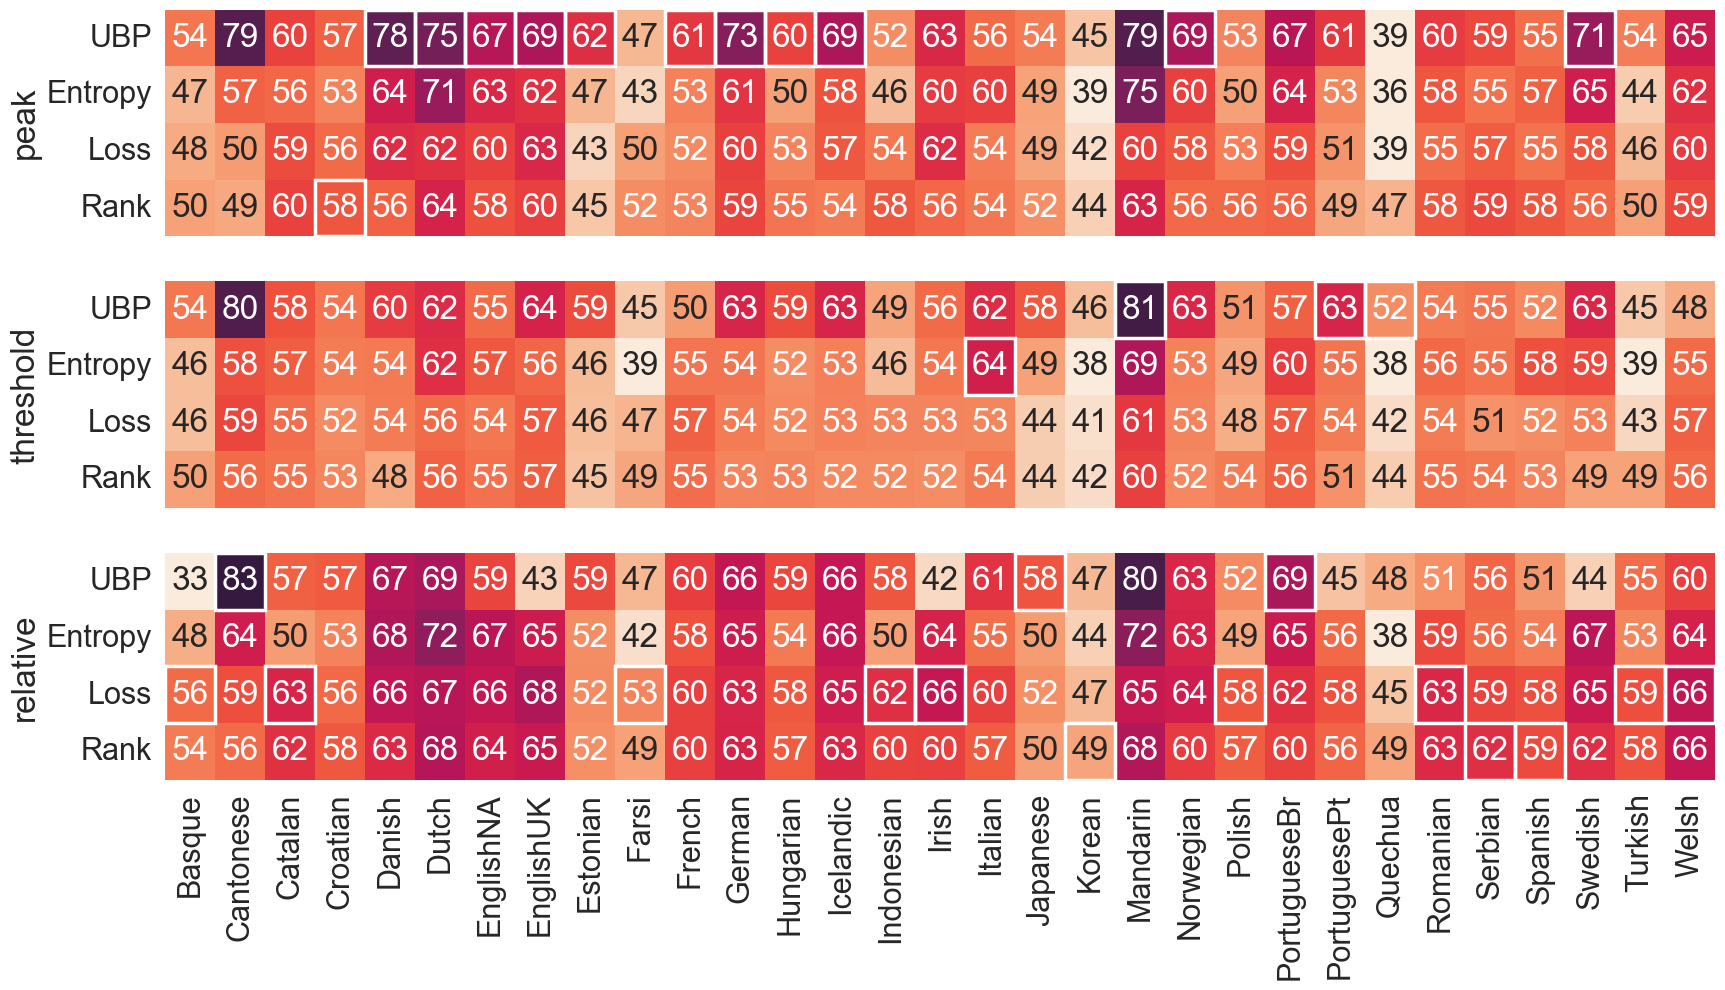
\includegraphics[width=0.99\linewidth]{Figures/15Phonology/tiny.png}
    \caption{Boundary placement F1 scores achieved by the models in the \textbf{Tiny} suite for each cue and segmentation strategy, with the highest score for each language highlighted.}
    \label{fig:15-tiny}
\end{figure*}

\begin{figure*}
    \centering
    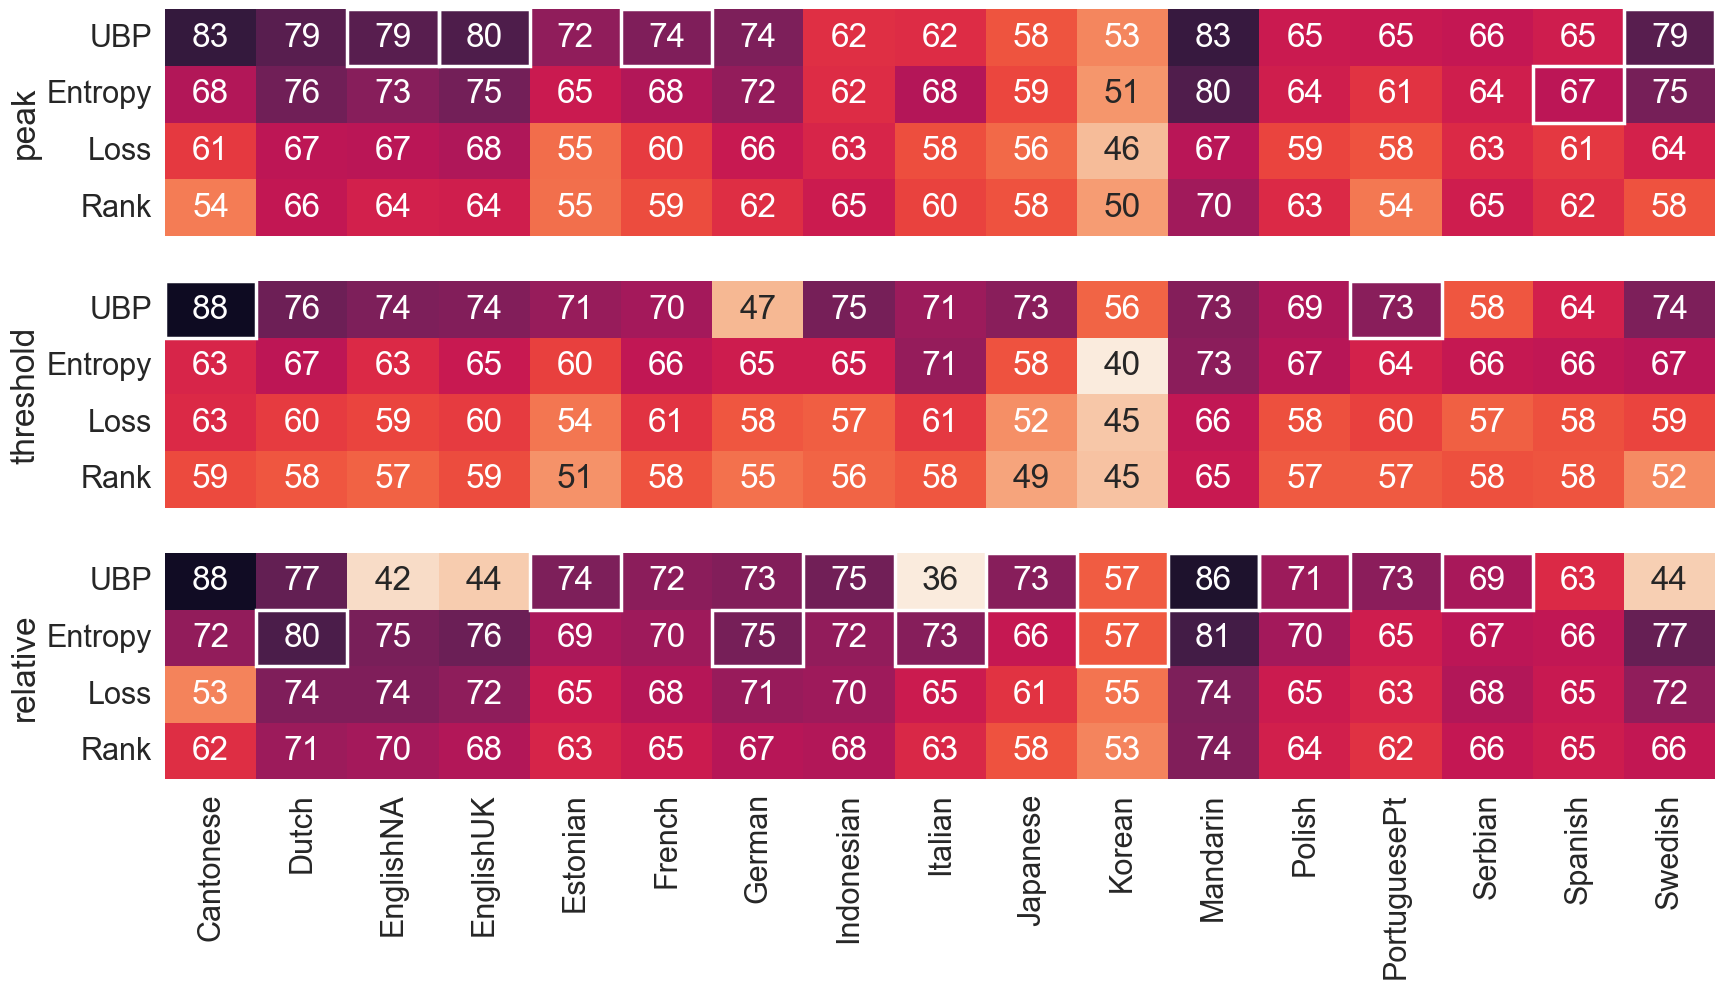
\includegraphics[width=0.99\linewidth]{Figures/15Phonology/small.png}
    \caption{Boundary placement F1 scores achieved by the models in the \textbf{Small} suite for each cue and segmentation strategy, with the highest score for each language highlighted.}
    \label{fig:15-small}
\end{figure*}

\begin{figure*}
    \centering
    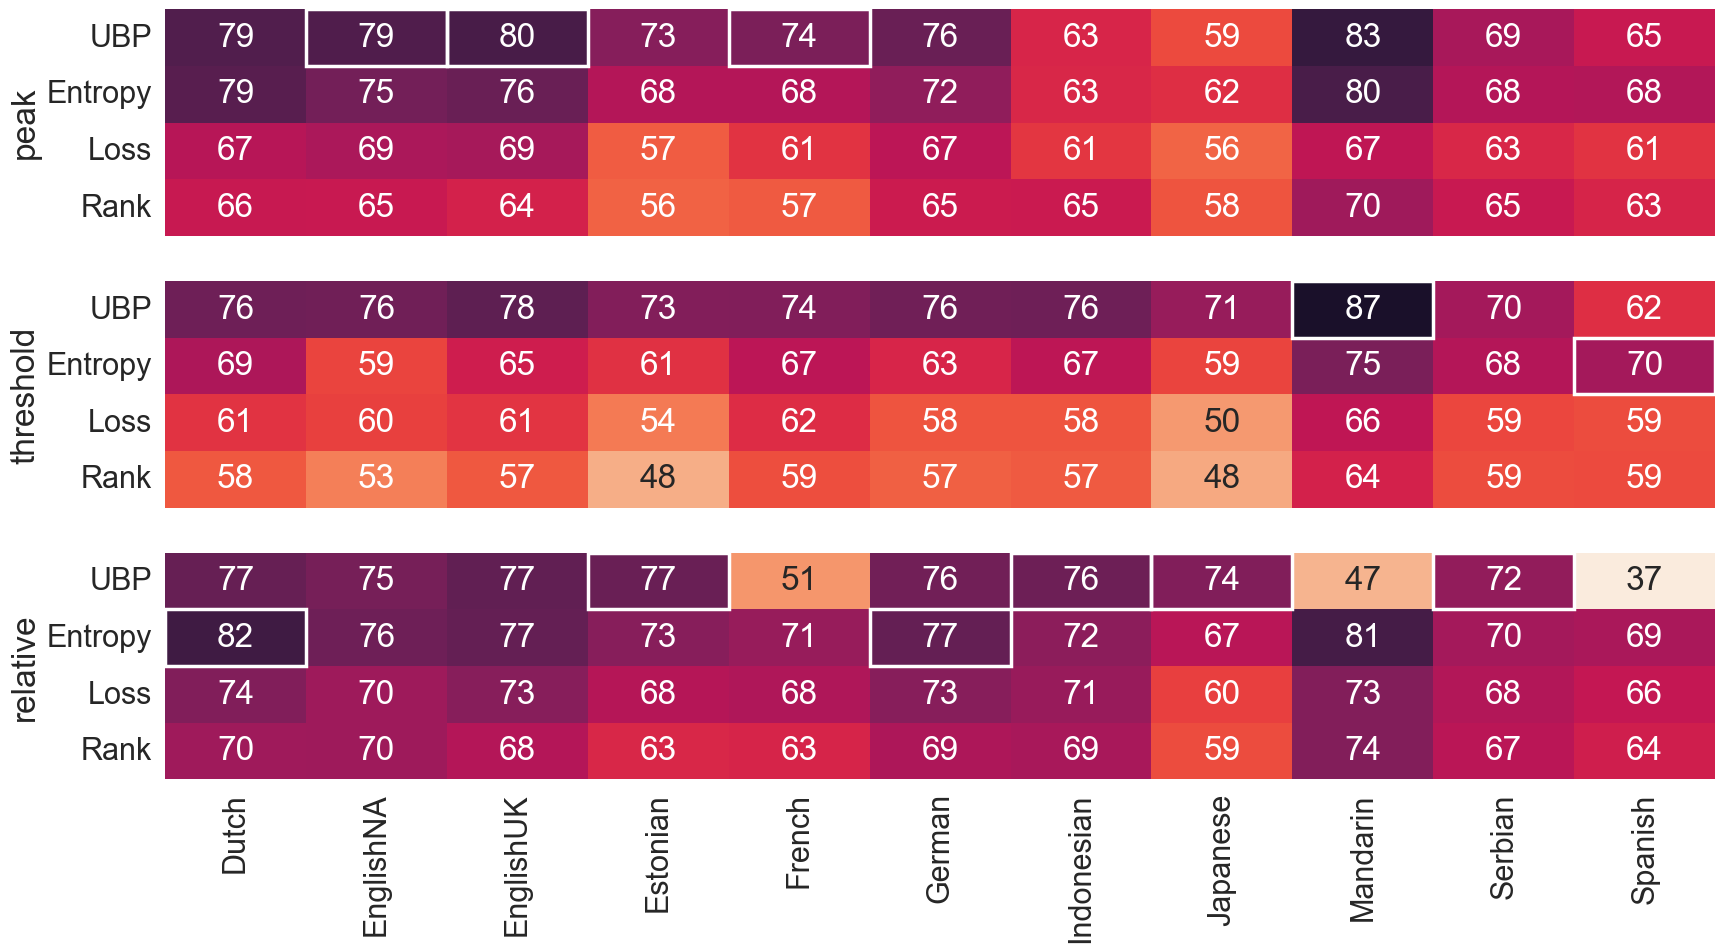
\includegraphics[width=0.99\linewidth]{Figures/15Phonology/medium.png}
    \caption{Boundary placement F1 scores achieved by the models in the \textbf{Medium} suite for each cue and segmentation strategy, with the highest score for each language highlighted.}
    \label{fig:15-medium}
\end{figure*}

\begin{figure*}
    \centering
    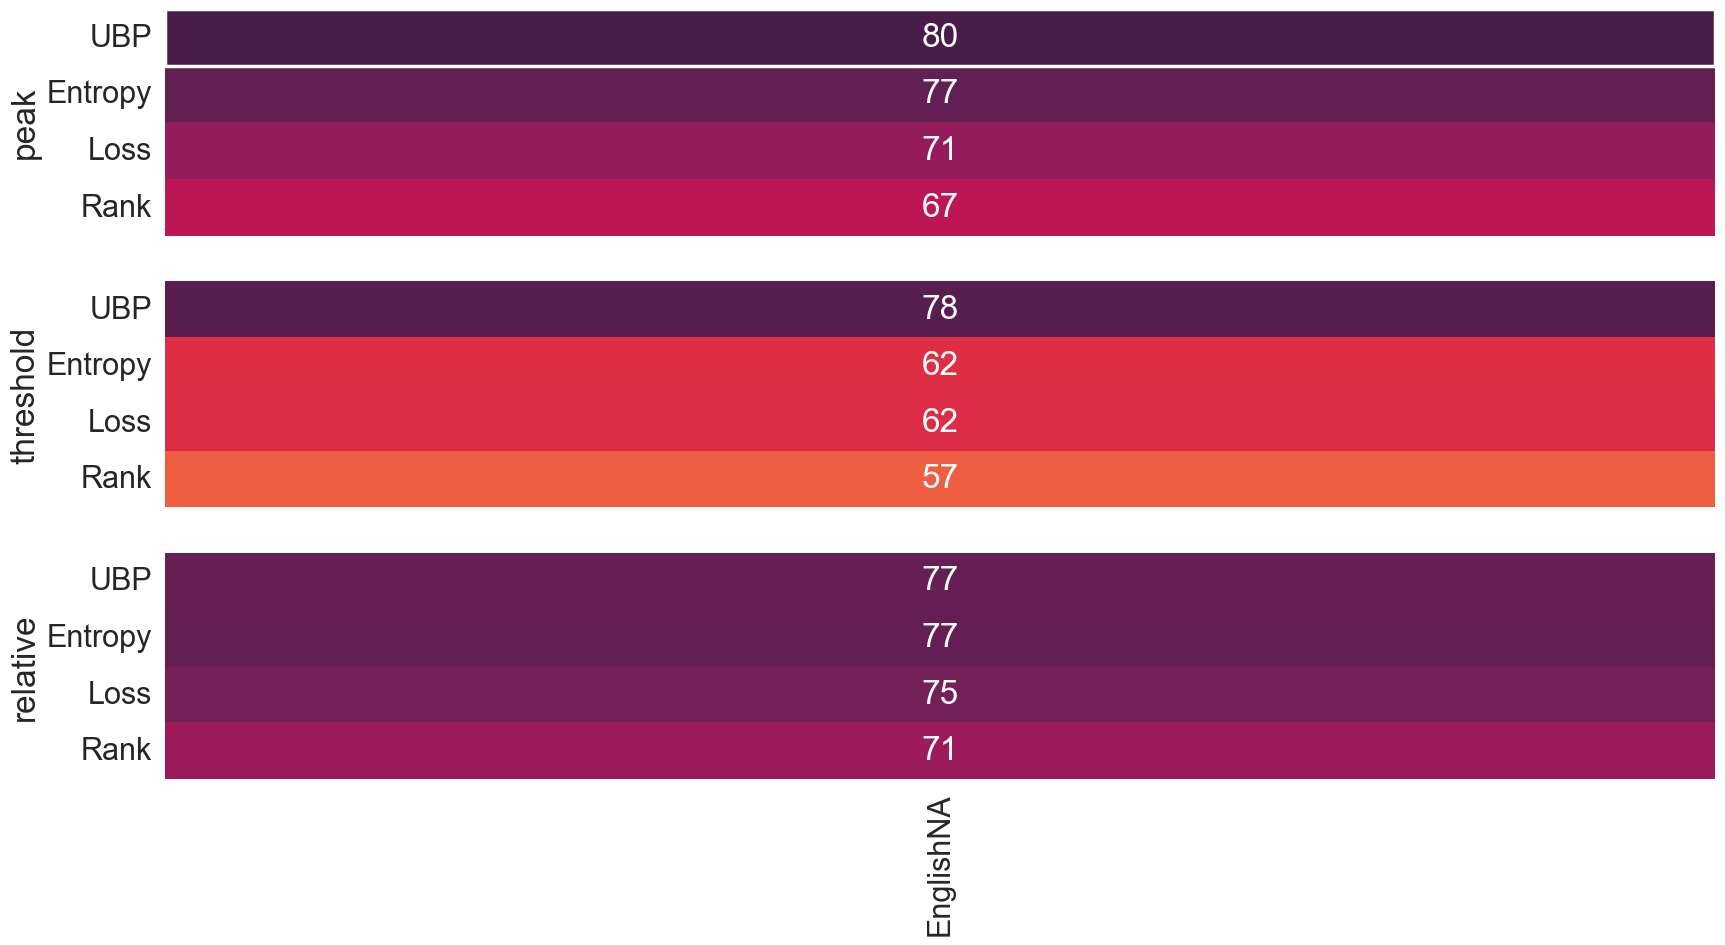
\includegraphics[width=0.99\linewidth]{Figures/15Phonology/large.png}
    \caption{Boundary placement F1 scores achieved by the models in the \textbf{Large} suite for each cue and segmentation strategy, with the highest score for each language highlighted.}
    \label{fig:15-large}
\end{figure*}


\begin{table*}[t]
    \centering
    \small
    \begin{tabular}{lllll}
    \toprule
    Language & 100k & 700k & 2M & 18M \\
    \midrule
    Basque & Loss (relative) &  &  &  \\
    Cantonese & UBP (relative) & UBP (threshold) &  &  \\
    Catalan & Loss (relative) &  &  &  \\
    Croatian & Rank (peak) &  &  &  \\
    Danish & UBP (peak) &  &  &  \\
    Dutch & UBP (peak) & Entropy (relative) & Entropy (relative) &  \\
    EnglishNA & UBP (peak) & UBP (peak) & UBP (peak) & UBP (peak) \\
    EnglishUK & UBP (peak) & UBP (peak) & UBP (peak) &  \\
    Estonian & UBP (peak) & UBP (relative) & UBP (relative) &  \\
    Farsi & Loss (relative) &  &  &  \\
    French & UBP (peak) & UBP (peak) & UBP (peak) &  \\
    German & UBP (peak) & Entropy (relative) & Entropy (relative) &  \\
    Hungarian & UBP (peak) &  &  &  \\
    Icelandic & UBP (peak) &  &  &  \\
    Indonesian & Loss (relative) & UBP (relative) & UBP (relative) &  \\
    Irish & Loss (relative) &  &  &  \\
    Italian & Entropy (threshold) & Entropy (relative) &  &  \\
    Japanese & UBP (relative) & UBP (relative) & UBP (relative) &  \\
    Korean & Rank (relative) & Entropy (relative) &  &  \\
    Mandarin & UBP (threshold) & UBP (relative) & UBP (threshold) &  \\
    Norwegian & UBP (peak) &  &  &  \\
    Polish & Loss (relative) & UBP (relative) &  &  \\
    PortugueseBr & UBP (relative) &  &  &  \\
    PortuguesePt & UBP (threshold) & UBP (threshold) &  &  \\
    Quechua & UBP (threshold) &  &  &  \\
    Romanian & Loss (relative) &  &  &  \\
    Serbian & Rank (relative) & UBP (relative) & UBP (relative) &  \\
    Spanish & Rank (relative) & Entropy (peak) & Entropy (threshold) &  \\
    Swedish & UBP (peak) & UBP (peak) &  &  \\
    Turkish & Loss (relative) &  &  &  \\
    Welsh & Loss (relative) &  &  &  \\
    \bottomrule
    \end{tabular}
    \caption{Best combination of boundary cue and segmentation strategy for each language and each suite.}
    \label{tab:15-bestcuesfull}
\end{table*}

\section{Significance Tests}\label{app:15-significance}

All word boundary probes for a particular language are trained and tested on the same evaluation set. We compute significance between two probes using McNemar’s Test \citep{McNemar_1947} over the predicted word boundaries for the evaluation set, with a significance threshold of $p<0.05$. The same procedure is used when comparing the unsupervised methods.

% \section{Qualitative Analysis of Threshold Segmentation}\label{app:15-qualitative}

% \begin{figure*}
%     \centering
%     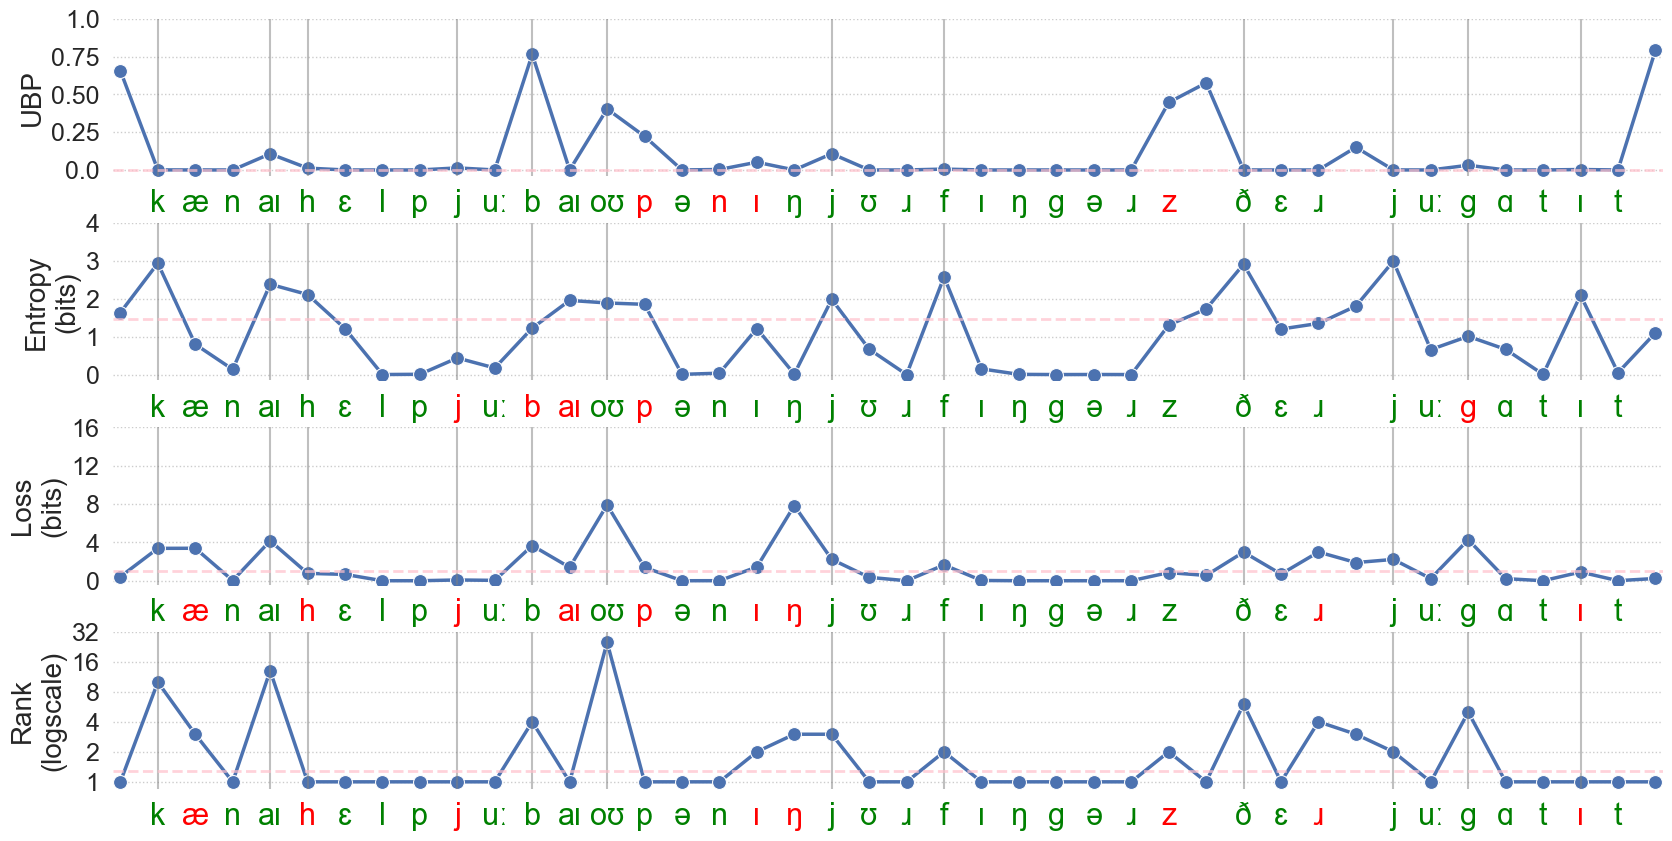
\includegraphics[width=\linewidth]{Figures/15Phonology/qualitative-threshold.png}
%     \caption{Per-phoneme boundary probability, entropy, loss and rank assigned by the Medium English model for the sequence of utterances ``can I help you by opening your fingers'', ``there'', ``you got it''. Spaces indicate utterance boundaries, vertical lines indicate gold word boundaries and phonemes are marked as green if they are correctly identified as word boundaries using the \textbf{threshold} segmentation strategy for that cue or if they follow an utterance boundary (red otherwise).}
%     \label{fig:15-qualitative-threshold}
% \end{figure*}

\section{Using Word Segmentation Cues for Subword Tokenization}\label{app:15-tokenizers}

We briefly explore the use of our unsupervised word boundary cues to create a subword tokenizer. Typically, the vocabularies for these tokenizers are generated using methods like Byte-Pair Encoding \citep{sennrich-etal-2016-bpe}, where the vocabulary initially consists of each individual byte, and pairs of bytes that frequently co-occur in a training dataset are `merged' into a new token, with this process repeated until a fixed vocabulary size is reached. We use the same principle, but base merges on the word boundary cues from a language model trained on the dataset.

Our method is as follows:

\begin{enumerate}
    \item We take a trained phoneme-level LM and compute either the UBP cue or the entropy cue at every position in the a given dataset. 
    \item We initialise our vocabulary $V$ to match the vocabulary of the phoneme LM (so it contains every phoneme plus the utterance boundary token).
    \item For every pair of tokens $x_i, x_j \in V$ that co-occur in the dataset, we compute the score for that pair by finding the average value of the word boundary cue at the position of the second token in the pair (e.g. for the pair \ttipa{D,E}, we find the value of the cue at every position where \ttipa{E} appears after \ttipa{D} and return the average). 
    \item We find the pair with the lowest score, create a new token $V_i+V_j$, add it to the vocabulary and apply the merge to every token in the dataset. The cue's value at the newly merged token is set to be the sum of the cue's value of the two tokens before the merging occurs. For the entropy cue this follows from the chain rule and for the UBP cue this results in the probability that \emph{either} original token was an utterance boundary.
    \item We repeat (2)-(3), adding new tokens and applying merges until a fixed vocabulary size is reached.
\end{enumerate}

Conceptually, creating merges using minimum average entropy will join highly predictable tokens together and result in tokens with comparable information and a uniformly dense signal that the model can learn from. Creating merges using the minimum average probability of an utterance boundary is similar, but instead tokens are joined according to the model's certainty that they do not cross an utterance boundary. 

In order to test this method, we use the phoneme-level LM trained by \citet{goriely2024babble} on a phonemized\zeb{fix?} version of the 100-million word BabyLM dataset \citep{choshen-et-al-2024-callforpapers-babylm2} and train subword tokenizers using a phonemized version of the 10-million word BabyLM dataset. We create two tokenizers with a vocabulary size of 16k using the UBP cue and the entropy cue. We compare these to the BPE tokenizer trained by \citet{goriely2024babble} on the same dataset, which also has a vocabulary size of 16k. Note that all three tokenizers are trained on a dataset without word boundaries, so it is possible for tokens to span word boundaries.

\citet{goriely2024babble} trained a large model using their BPE tokenizer on the 100-million word BabyLM dataset and evaluated their results on two linguistic benchmarks, BLIMP \citep{warstadt-2020-blimp} and BabySLM \citep{lavechin}. We train and evaluate a model using the same procedure but replace their tokenizer for ours. 

\begin{table}[t]
    \centering
    \begin{tabular}{lccc}
        \toprule
        Tokenizer & \rotatebox[origin=l]{90}{BLIMP} & \rotatebox[origin=l]{90}{BabySLM Syntactic} & \rotatebox[origin=l]{90}{BabySLM Lexical} \\
        \midrule
        BPE & 71.7 & 74.7 & 71.2 \\
        Entropy & 72.7 & 77.6 & 81.3 \\
        UBP & 72.6 & 85.6 & 84.4 \\
        \bottomrule
    \end{tabular}
    \caption{BLIMP and BabySLM scores achieved by a GPT-2 model trained on the BabyLM dataset. We compare BPE to our subword method, where merges are assigned using either entropy or UBP as a cue. BPE results are taken from \citet{goriely2024babble}.}
    \label{tab:15-tokenizerresults}
\end{table}

The results of this experiment are provided in \cref{tab:15-tokenizerresults}. We find that our two tokenizers improve all three scores compared to the BPE tbut instead okenizer with the UBP cue leading to a particularly large improvement for the BabySLM syntactic score.

Our method is similar to \citet{pagnoni2024byte}, who calculate the entropy cue over bytes using a small byte-level LLM, and use either a \textit{global constraint} (corresponding to our threshold segmentation strategy) or a \textit{monotonic constraint} (corresponding to our relative segmentation strategy) in order to group bytes into latent `patches'. These patches are then fed into the main model, a large transformer, and the encoded patches are `unpatched' and fed back into the byte-level LLM to predict the next byte. Future work should investigate whether their method is improved by using the cues explored in this study. When training with word boundaries, the prediction of the space character (or other word boundary characters) could also be used to group bytes.


\section{Related Work}

\citet{bunzeck-etal-2025-small} use a similar approach in order to compare grapheme LMs to phoneme LMs. They also use two probing tasks to examine the representations of sentences; age prediction and rhyme prediction.